\documentclass[a4paper,12pt]{report}
\usepackage[spanish]{babel}
\usepackage[utf8]{inputenc}
\usepackage{graphicx, csquotes, longtable, array, booktabs, xparse, float, titlesec, enumitem, dingbat, soul, multicol, listings, wrapfig}
\usepackage[dvipsnames]{xcolor}
\usepackage[margin=2cm]{geometry}

% Añadir la bibliografía
%\usepackage[backend=biber, style=numeric, sorting=ynt]{biblatex}
%\addbibresource{TFG.bib}

% Cambia el color de los links
\usepackage{hyperref}
\hypersetup{hidelinks}

% Generamos un comando para saltar pagina con las secciones
\NewDocumentCommand{\cpsection}{s o m}{%
  \clearpage
  \IfBooleanTF{#1}
    {\section*{#3}}
    {%
      \IfNoValueTF{#2}
        {\section{#3}}
        {\section[#2]{#3}}%
    }%
}

\NewDocumentCommand{\cpsubsection}{s o m}{%
  \clearpage
  \IfBooleanTF{#1}
    {\subsection*{#3}}
    {%
      \IfNoValueTF{#2}
        {\subsection{#3}}
        {\subsection[#2]{#3}}%
    }%
}

% Elimina la palabra 'Capítulo' de los títulos de los capítulos
\titleformat{\chapter}[display]
  {\normalfont\bfseries}{}{0pt}{\Huge\thechapter.\space}

\titleformat{name=\chapter,numberless}[display]
  {\normalfont\bfseries}{}{0pt}{\Huge}

\titlespacing*{\chapter}{0pt}{-50pt}{20pt}

% Personalización del índice de listados
\renewcommand{\lstlistingname}{Código}  % Cambiar el nombre de 'Listing' a 'Código'
\renewcommand{\lstlistlistingname}{Índice de códigos}

% Añade numeración a los subsubsections y los añade al índice
\setcounter{secnumdepth}{4}
\setcounter{tocdepth}{4}

% Idioma predeterminado (Español)
\selectlanguage{spanish}

\begin{document}
  \begin{titlepage}
      \centering
      
\includegraphics[width=0.6\textwidth]{./.img/logo.jpg}\\
      \vspace{1cm}
      \Large Ingeniería Informática de Gestión y Sistemas de Información\\
      \vspace{3cm}
      \Huge Desarrollo Avanzado de Software\\
      \vspace{0.5cm}
      \huge \textbf{LibreBook}\\
      \vspace{7.5cm}
      \Large Estudiante:\\
      \vspace{0.2cm}
      \large Gabiña Barañano, Xabier\\
      \vspace{1cm}
      \vfill
      \today
  \end{titlepage}
  \tableofcontents
  \listoffigures
  \chapter{Introducción}
    \paragraph*{}{
      LibreBook es una aplicación móvil para Android diseñada para los amantes de la lectura. Es una plataforma que permite a los usuarios crear una biblioteca personal digital donde pueden registrar, organizar y seguir su progreso en los libros que están leyendo o desean leer.
    }
    \paragraph*{}{
      La aplicación está desarrollada completamente en Java y sigue las mejores prácticas de desarrollo para Android, incluyendo el uso de Room para la persistencia de datos, arquitectura MVVM, y componentes de la biblioteca de Material Design para ofrecer una interfaz moderna y funcional.\\
      El repositorio de la aplicación se encuentra en GitHub y está disponible para su descarga y uso bajo la licencia MIT.
    }
    \begin{center}
      %Link al repositorio
        \color{blue}\href{https://github.com/Xabierland/DAS-Proyecto}{Repositorio de la aplicación}
    \end{center}
    \paragraph*{}{
      Además en el repositorio, tambien esta disponible en GitHub el binario de la aplicación en formato apk para su descarga e instalación en dispositivos Android.
    }
    \begin{center}
      %Link al binario
        \color{blue}\href{}{Archivo APK de la aplicación}
    \end{center}
    \paragraph*{}{
      En la aplicación existen por defecto unicamente 10 libros.
      \begin{multicols}{2}
        \begin{enumerate}
          \item Crimen y Castigo
          \item Los Hermanos Karamazov
          \item El Idiota
          \item Memorias del Subsuelo
          \item El Jugador
          \item Los Demonios
          \item Humillados y Ofendidos
          \item El eterno marido
          \item Noches Blancas
          \item El doble
        \end{enumerate}
      \end{multicols}
      Todos de Dostoievski. Tenlo en cuenta a la hora de buscar los libros ya que no se pueden añadir libros directamente desde la aplicación.
    }
    \paragraph*{}{
      La aplicación cuenta con dos cuentas de usuario por defectos:
      \begin{itemize}
        \item \textbf{Administrador}
          \begin{itemize}
            \item Email: admin@xabierland.com
            \item Contraseña: admin
          \end{itemize}
        \item \textbf{Xabier}
          \begin{itemize}
            \item Email: xabierland@gmail.com
            \item Contraseña: 123456
          \end{itemize}
      \end{itemize}
      No obstante, se pueden crear nuevas cuentas de usuario mediante el registro en la aplicación.
    }
  \chapter{Objetivos}
    \section{Elementos obligatorios}
      \begin{itemize}
        \item \textbf{Uso de ListView+CardView personalizado o de RecyclerView+CardView para mostrar listados de elementos con diferentes características.}
        \begin{itemize}
          \item En la actividad principal (MainActivity.java) se muestra una lista de cuatro libros aleatorios de la base de datos mediante RecyclerView.
          \item En la actividad de búsqueda (SearchActivity.java), dependiendo de la posición del switch, se muestra una lista de libros o de usuarios usando el mismo RecyclerView.
          \item En la actividad del perfil (ProfileActivity.java), se muestran tres listas horizontales de libros separadas por categoría (leyendo, por leer, leídos) mediante RecyclerView.
          \item Todas estas RecyclerViews usan un adaptador personalizado (BookCardAdapter.java, UsuarioAdapter, LibroAdapter) para mostrar los CardViews con la información de cada elemento.
        \end{itemize}
        \item \textbf{Usar una base de datos local, para listar, añadir y modificar elementos y características de cada elemento.}
        \begin{itemize}
          \item Se implementa Room para gestionar la base de datos SQLite (AppDatabase.java).
          \item Se han creado entidades como Libro.java, Usuario.java y UsuarioLibro.java con sus respectivas relaciones.
          \item Los DAOs correspondientes (LibroDao.java, UsuarioDao.java, UsuarioLibroDao.java) contienen métodos para insertar, actualizar, eliminar y consultar datos.
          \item Los repositorios (LibroRepository.java, UsuarioRepository.java, BibliotecaRepository.java) proporcionan una capa adicional de abstracción para el acceso a datos.
        \end{itemize}
        \item \textbf{Uso de diálogos.}
        \begin{itemize}
          \item En SettingsActivity.java se implementan diálogos para cambiar el tema y el idioma de la aplicación.
          \item En BookDetailActivity.java se utiliza un diálogo personalizado (dialog\_add\_book.xml) para añadir libros a la biblioteca y elegir su estado (leído, leyendo, por leer).
          \item En BaseActivity.java se muestra un diálogo de confirmación al querer cerrar sesión.
          \item En ProfileActivity.java se implementa un diálogo para solicitar permisos de acceso a la galería.
          \item Se utilizan diálogos de carga (dialog\_loading.xml) durante las operaciones de busqueda que puedan llevar tiempo.
        \end{itemize}
        \item \textbf{Usar notificaciones locales.}
        \begin{itemize}
          \item En RegisterActivity.java, tras el registro exitoso de un usuario, se muestra una notificación de bienvenida.
          \item La clase NotificationUtils.java implementa métodos para crear el canal de notificaciones y mostrar la notificación.
        \end{itemize}
        \item \textbf{Control de la pila de actividades.}
        \begin{itemize}
          \item En BaseActivity.java, método handleNavigationItemSelected(), se controla la navegación entre actividades.
          \item Se utilizan flags como FLAG\_ACTIVITY\_CLEAR\_TOP y FLAG\_ACTIVITY\_SINGLE\_TOP para gestionar la pila de actividades.
          \item Se comprueba si ya estamos en la actividad a la que queremos ir para evitar crear instancias innecesarias.
          \item En los métodos setLanguageMode() y setThemeMode() se reinicia la pila de actividades para aplicar los cambios globalmente.
          \item En métodos como logoutUser() se controla correctamente el regreso a la actividad principal.
          \end{itemize}
      \end{itemize}
    \cpsection{Elementos opcionales}
      \begin{itemize}
        \item \textbf{Permitir que una misma funcionalidad se comporte de manera distinta dependiendo de la orientación (o del tamaño) del dispositivo mediante el uso de Fragments.}
        \begin{itemize}
          \item En la actividad de detalle del libro (BookDetailActivity.java) se utilizan dos fragments: BookInfoFragment y BookActionsFragment.
          \item En orientación vertical (layout activity\_book\_detail.xml), los fragments se muestran uno sobre otro.
          \item En orientación horizontal (layout-land/activity\_book\_detail.xml), los fragments se muestran uno al lado del otro, aprovechando mejor el espacio horizontal.
          \item Los fragments permiten una mejor separación de responsabilidades: BookInfoFragment muestra la información detallada del libro, mientras que BookActionsFragment maneja las acciones que el usuario puede realizar.
        \end{itemize}
        \item \textbf{Hacer la aplicación multiidioma y añadir la opción de cambiar de idioma en la propia aplicación.}
        \begin{itemize}
          \item La aplicación soporta tres idiomas: inglés (values/strings.xml), español (values-es/strings.xml) y euskera (values-eu/strings.xml).
          \item En SettingsActivity.java se implementa la opción para cambiar el idioma mediante un diálogo.
          \item En BaseActivity.java, los métodos loadLocale(), applyLanguage() y setLanguageMode() gestionan el cambio de idioma.
          \item El idioma seleccionado se guarda en SharedPreferences y se aplica en toda la aplicación.
        \end{itemize}
        \item \textbf{Uso de ficheros de texto.}
        \begin{itemize}
          \item En ProfileActivity.java se implementa la funcionalidad para guardar y cargar imágenes de perfil como archivos en el almacenamiento interno.
          \item En el método saveProfileImage() se guarda la imagen de perfil seleccionada como un archivo JPEG.
          \item En DatabaseInitializer.java se crean archivos de imagen para los usuarios predeterminados.
          \item En el método updateNavigationHeader() de BaseActivity.java se cargan las imágenes de perfil desde archivos.
        \end{itemize}
        \item \textbf{Uso de Preferencias, para guardar las preferencias del usuario en cuanto a mostrar/esconder cierta información, elegir colores para la aplicación, o cualquier otra cosa relacionada con la visualización de la aplicación.}
        \begin{itemize}
          \item En BaseActivity.java se guardan preferencias para el idioma y el tema seleccionados.
          \item En LoginActivity.java y RegisterActivity.java se guardan datos de sesión del usuario.
          \item Las preferencias permiten persistir la configuración elegida por el usuario entre sesiones.
        \end{itemize}
        \item \textbf{Crear estilos y temas propios, para personalizar fondos, botones, etc.}
        \begin{itemize}
          \item Se han definido temas personalizados en values/themes.xml y values-night/themes.xml.
          \item Se han creado estilos específicos para el modo claro (Theme.LibreBook.Light) y el modo oscuro (Theme.LibreBook.Dark).
          \item Se han definido atributos personalizados en attrs.xml como backgroundColor, cardBackgroundColor y textColor.
          \item Se utilizan drawables personalizados como rounded\_background.xml para dar estilo a elementos visuales.
          \item Los temas aplican colores consistentes a lo largo de toda la aplicación.
        \end{itemize}
        \item \textbf{Usar intents implícitos para abrir otras aplicaciones, contactos, etc.}
        \begin{itemize}
          \item En ProfileActivity.java se utiliza un intent implícito para abrir la galería de imágenes (ACTION\_PICK).
          \item En el método onRequestPermissionsResult() se utiliza un intent implícito para abrir los ajustes de la aplicación cuando se deniegan permisos.
          \item El intent Intent(android.provider.Settings.ACTION\_APPLICATION\_DETAILS\_SETTINGS) permite al usuario ir directamente a los ajustes de permisos de la aplicación.
          \item En ImageLoader.java se accede implícitamente a recursos de internet para cargar imágenes desde URLs.
        \end{itemize}
        \item \textbf{Añadir una barra de herramientas (ToolBar) personalizada en la aplicación así como un panel de navegación (Navigation Drawer)}
        \begin{itemize}
          \item En BaseActivity.java se implementa un Toolbar personalizado que se hereda en todas las actividades.
          \item El método setupToolbar() configura la barra de herramientas con el título específico de cada actividad.
          \item Se implementa un Navigation Drawer (panel lateral de navegación) en el método setupDrawer().
          \item El Navigation Drawer incluye un encabezado personalizado (nav\_header\_main.xml) que muestra información del usuario.
          \item El menú del Navigation Drawer (drawer\_menu.xml) incluye opciones diferentes según el estado de autenticación del usuario.
        \end{itemize}
      \end{itemize}
  \chapter{Descripción de la aplicación}
    \section{Clases}
      \begin{figure}[H]
        \centering
        \href{https://raw.githubusercontent.com/Xabierland/DAS-Proyecto/refs/heads/main/Documentation/.img/diagrama-clases.svg}{%}
          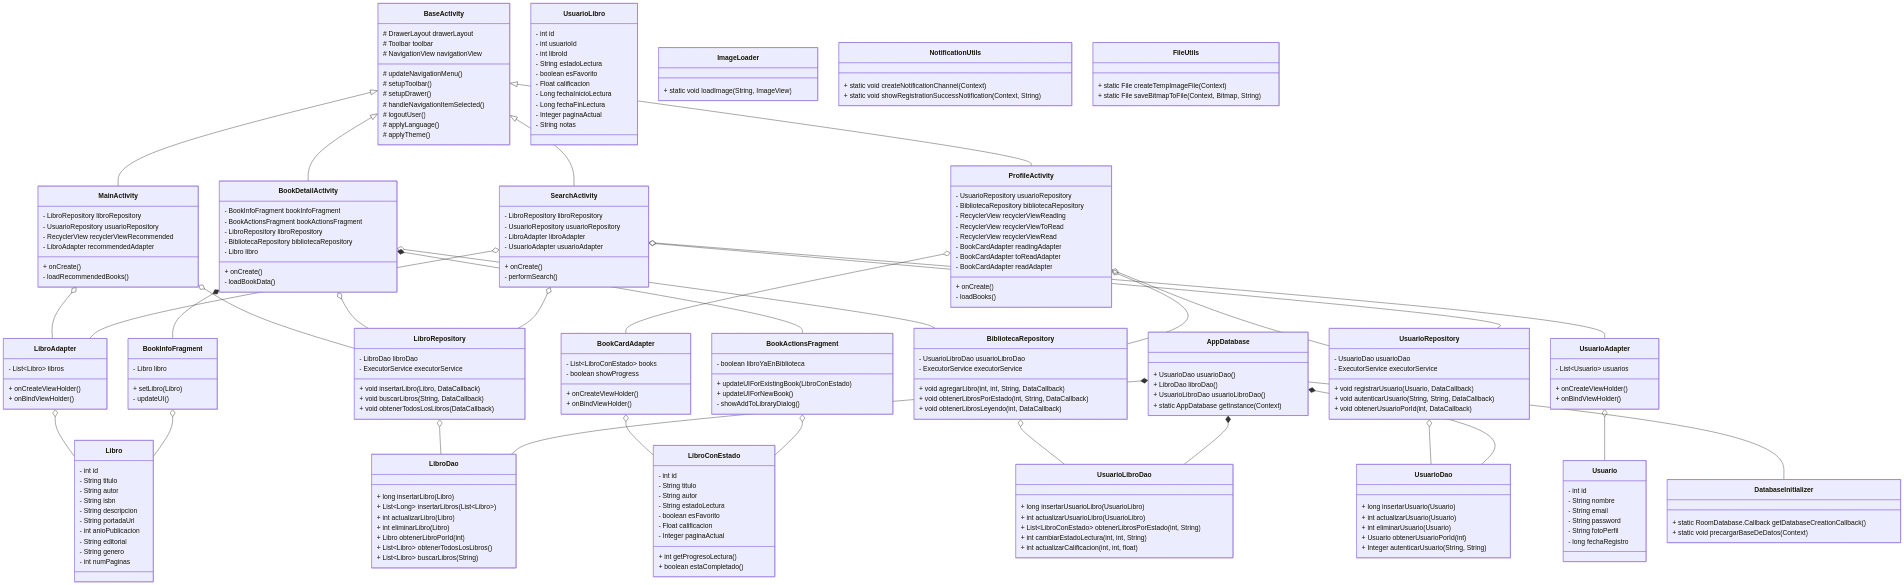
\includegraphics[width=0.9\textwidth]{.img/diagrama-clases.png} 
        }
        \caption{Diagrama de clases de la aplicación LibreBook}
        \label{fig:diagrama-clases}
      \end{figure}
      La aplicación está estructurada siguiendo un patrón arquitectónico basado en capas con una clara separación de responsabilidades:
      \subsection{Activities}
      \begin{itemize}
        \item \textbf{BaseActivity}: Clase abstracta que implementa la funcionalidad común a todas las actividades, como la barra de herramientas, el menú lateral, la gestión de idiomas y temas, y el control de sesión.
        \item \textbf{MainActivity}: Actividad principal que muestra la pantalla de inicio con libros recomendados y mensajes de bienvenida personalizados.
        \item \textbf{LoginActivity}: Gestiona la autenticación de usuarios existentes, validando credenciales y estableciendo la sesión.
        \item \textbf{RegisterActivity}: Maneja el registro de nuevos usuarios, incluyendo validación de datos y creación de cuentas.
        \item \textbf{BookDetailActivity}: Muestra los detalles de un libro específico mediante dos fragments y permite realizar acciones como añadir a la biblioteca o valorar.
        \item \textbf{ProfileActivity}: Presenta el perfil del usuario con sus estadísticas de lectura y bibliotecas organizadas por estado (leyendo, por leer, leídos).
        \item \textbf{SearchActivity}: Permite buscar libros o usuarios mediante un sistema de filtrado en tiempo real.
        \item \textbf{SettingsActivity}: Ofrece opciones para personalizar la aplicación, como cambiar el idioma o el tema.
      \end{itemize}
      \subsection{Fragments}
      \begin{itemize}
        \item \textbf{BookInfoFragment}: Muestra la información detallada de un libro (portada, título, autor, descripción, etc.).
        \item \textbf{BookActionsFragment}: Presenta las acciones que el usuario puede realizar con un libro (añadir a biblioteca, calificar, revisar, actualizar estado).
      \end{itemize}
      \subsection{Adaptadores}
      \begin{itemize}
        \item \textbf{LibroAdapter}: Adaptador para mostrar listas de libros en formato vertical usando CardView.
        \item \textbf{BookCardAdapter}: Adaptador especializado para mostrar libros en formato horizontal con información adicional sobre progreso de lectura.
        \item \textbf{UsuarioAdapter}: Adaptador para mostrar listas de usuarios con su información básica.
      \end{itemize}
      \subsection{Modelos y Entidades}
      \begin{itemize}
        \item \textbf{Libro}: Entidad que representa un libro con sus atributos (título, autor, ISBN, descripción, etc.).
        \item \textbf{Usuario}: Entidad que representa un usuario de la aplicación (nombre, email, contraseña, foto de perfil).
        \item \textbf{UsuarioLibro}: Entidad de relación entre usuarios y libros que almacena estado de lectura, calificaciones, notas, etc.
        \item \textbf{LibroConEstado}: Clase POJO (Plain Old Java Object) que combina información de un libro y su estado en la biblioteca de un usuario.
      \end{itemize}
      \subsection{Data Access Objects (DAOs)}
      \begin{itemize}
        \item \textbf{LibroDao}: Interfaz que define operaciones de acceso a datos para la entidad Libro.
        \item \textbf{UsuarioDao}: Interfaz para operaciones de acceso a datos relacionadas con usuarios.
        \item \textbf{UsuarioLibroDao}: Interfaz para operaciones de acceso a datos de la relación usuario-libro.
      \end{itemize}
      \subsection{Repositorios}
      \begin{itemize}
        \item \textbf{LibroRepository}: Encapsula la lógica de acceso a datos para libros, proporcionando un API limpia a las actividades.
        \item \textbf{UsuarioRepository}: Gestiona el acceso a datos para usuarios, incluyendo operaciones como registro y autenticación.
        \item \textbf{BibliotecaRepository}: Maneja las operaciones relacionadas con la biblioteca personal de un usuario.
      \end{itemize}
      \subsection{Utilidades}
      \begin{itemize}
        \item \textbf{ImageLoader}: Utilidad para cargar imágenes desde URLs (portadas de libros).
        \item \textbf{FileUtils}: Utilidad para operaciones con archivos, especialmente para gestionar imágenes de perfil.
        \item \textbf{NotificationUtils}: Gestiona la creación y visualización de notificaciones locales.
        \item \textbf{DatabaseInitializer}: Responsable de precargar datos iniciales en la base de datos.
      \end{itemize}
    \cpsection{Base de datos}
      \begin{figure}[H]
        \centering
        \href{https://raw.githubusercontent.com/Xabierland/DAS-Proyecto/refs/heads/main/Documentation/.img/diagrama-bd.svg}{%
          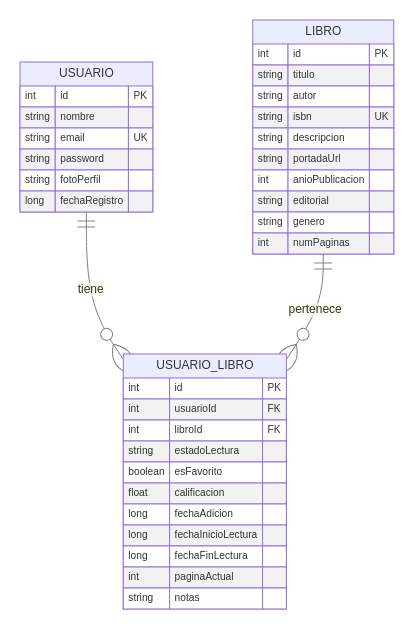
\includegraphics[width=0.4\textwidth]{.img/diagrama-bd.png}
        }
        \caption{Diagrama de la base de datos de la aplicación LibreBook}
        \label{fig:diagrama-bd}
      \end{figure}
      La aplicación utiliza Room como una capa de abstracción sobre SQLite para proporcionar un acceso más sencillo y seguro a los datos.
      \subsection{Estructura de la base de datos}
        La base de datos está definida por la clase \textbf{AppDatabase}, que extiende de RoomDatabase, y contiene las siguientes entidades:
        \begin{itemize}
          \item \textbf{Entidad Libro}: Almacena información completa sobre libros.
          \begin{itemize}
            \item \textbf{Atributos principales}: id, titulo, autor, isbn, descripcion, portadaUrl, anioPublicacion, editorial, genero, numPaginas.
            \item \textbf{Índices}: ISBN es un campo único indexado para búsquedas eficientes.
          \end{itemize}
          \item \textbf{Entidad Usuario}: Almacena datos de los usuarios registrados.
          \begin{itemize}
            \item \textbf{Atributos principales}: id, nombre, email, password, fotoPerfil, fechaRegistro.
            \item \textbf{Índices}: email es un campo único indexado para prevenir duplicados y facilitar búsquedas.
          \end{itemize}
          \item \textbf{Entidad UsuarioLibro}: Tabla de relación muchos a muchos que conecta usuarios con libros y almacena metadatos de la relación.
          \begin{itemize}
            \item \textbf{Atributos principales}: id, usuarioId, libroId, estadoLectura, esFavorito, calificacion, fechaAdicion, fechaInicioLectura, fechaFinLectura, paginaActual, notas.
            \item \textbf{Claves foráneas}: usuarioId referencia a Usuario.id, libroId referencia a Libro.id.
            \item \textbf{Índices}: Índice compuesto sobre (usuarioId, libroId) para asegurar unicidad y optimizar consultas.
          \end{itemize}
        \end{itemize}
      \subsection{Operaciones principales}
        La base de datos soporta las siguientes operaciones a través de los DAOs:
        \begin{itemize}
          \item \textbf{Operaciones CRUD básicas}:
            \begin{itemize}
              \item Inserción, actualización y eliminación de libros, usuarios y relaciones.
              \item Consultas por identificador, ISBN, email, etc.
              \item Listados completos de entidades.
            \end{itemize}
          \item \textbf{Consultas específicas}:
            \begin{itemize}
              \item Búsqueda de libros por título o autor (mediante LIKE).
              \item Filtrado por género o autor.
              \item Obtención de listas de géneros y autores únicos.
              \item Autenticación de usuarios (validación de email y contraseña).
              \item Búsqueda de usuarios por nombre o email.
            \end{itemize}
          \item \textbf{Consultas relacionales}:
            \begin{itemize}
              \item Obtención de todos los libros de un usuario, opcionalmente filtrados por estado de lectura.
              \item Obtención de libros favoritos.
              \item Cálculo de estadísticas de lectura (conteo por estado, calificación promedio).
            \end{itemize}
        \end{itemize}
      \subsection{Inicialización y precarga}
        La clase \textbf{DatabaseInitializer} se encarga de:
        \begin{itemize}
          \item Crear la base de datos si no existe.
          \item Precargar 10 libros de Dostoievski para tener datos de ejemplo.
          \item Crear usuarios predeterminados (Administrador y Xabier).
          \item Establecer relaciones iniciales entre el usuario Xabier y algunos libros con diferentes estados de lectura, calificaciones y notas.
        \end{itemize}
      \subsection{Transacciones y concurrencia}
        \begin{itemize}
          \item Todas las operaciones de base de datos se realizan en hilos secundarios mediante ExecutorService para no bloquear la interfaz de usuario.
          \item Los callbacks permiten notificar a la UI cuando las operaciones se completan.
          \item Room maneja automáticamente las transacciones para asegurar la integridad de los datos.
        \end{itemize}
        \chapter{Manual de usuario}
        \setlength{\intextsep}{2pt}        % Espacio entre texto y figuras
        \setlength{\abovecaptionskip}{1pt}  % Espacio sobre las leyendas
        \setlength{\belowcaptionskip}{1pt}  % Espacio bajo las leyendas
        \setlength{\parskip}{2pt}          % Espacio entre párrafos
        \setlength{\topsep}{1pt}           % Espacio en listas y entornos
        \begin{multicols}{2}
        % Ajustes de espaciado global para esta sección
        \vspace{-1.5em}  % Reduce espacio después del título del capítulo
        \section{Inicio}
        \vspace{-0.8em}  % Reduce espacio después del título de sección
        Al abrir la aplicación, se muestra la pantalla de inicio con libros recomendados y un mensaje de bienvenida. Puedes acceder al menú lateral mediante el icono de hamburguesa.
        
        \begin{figure}[H]
          \centering
          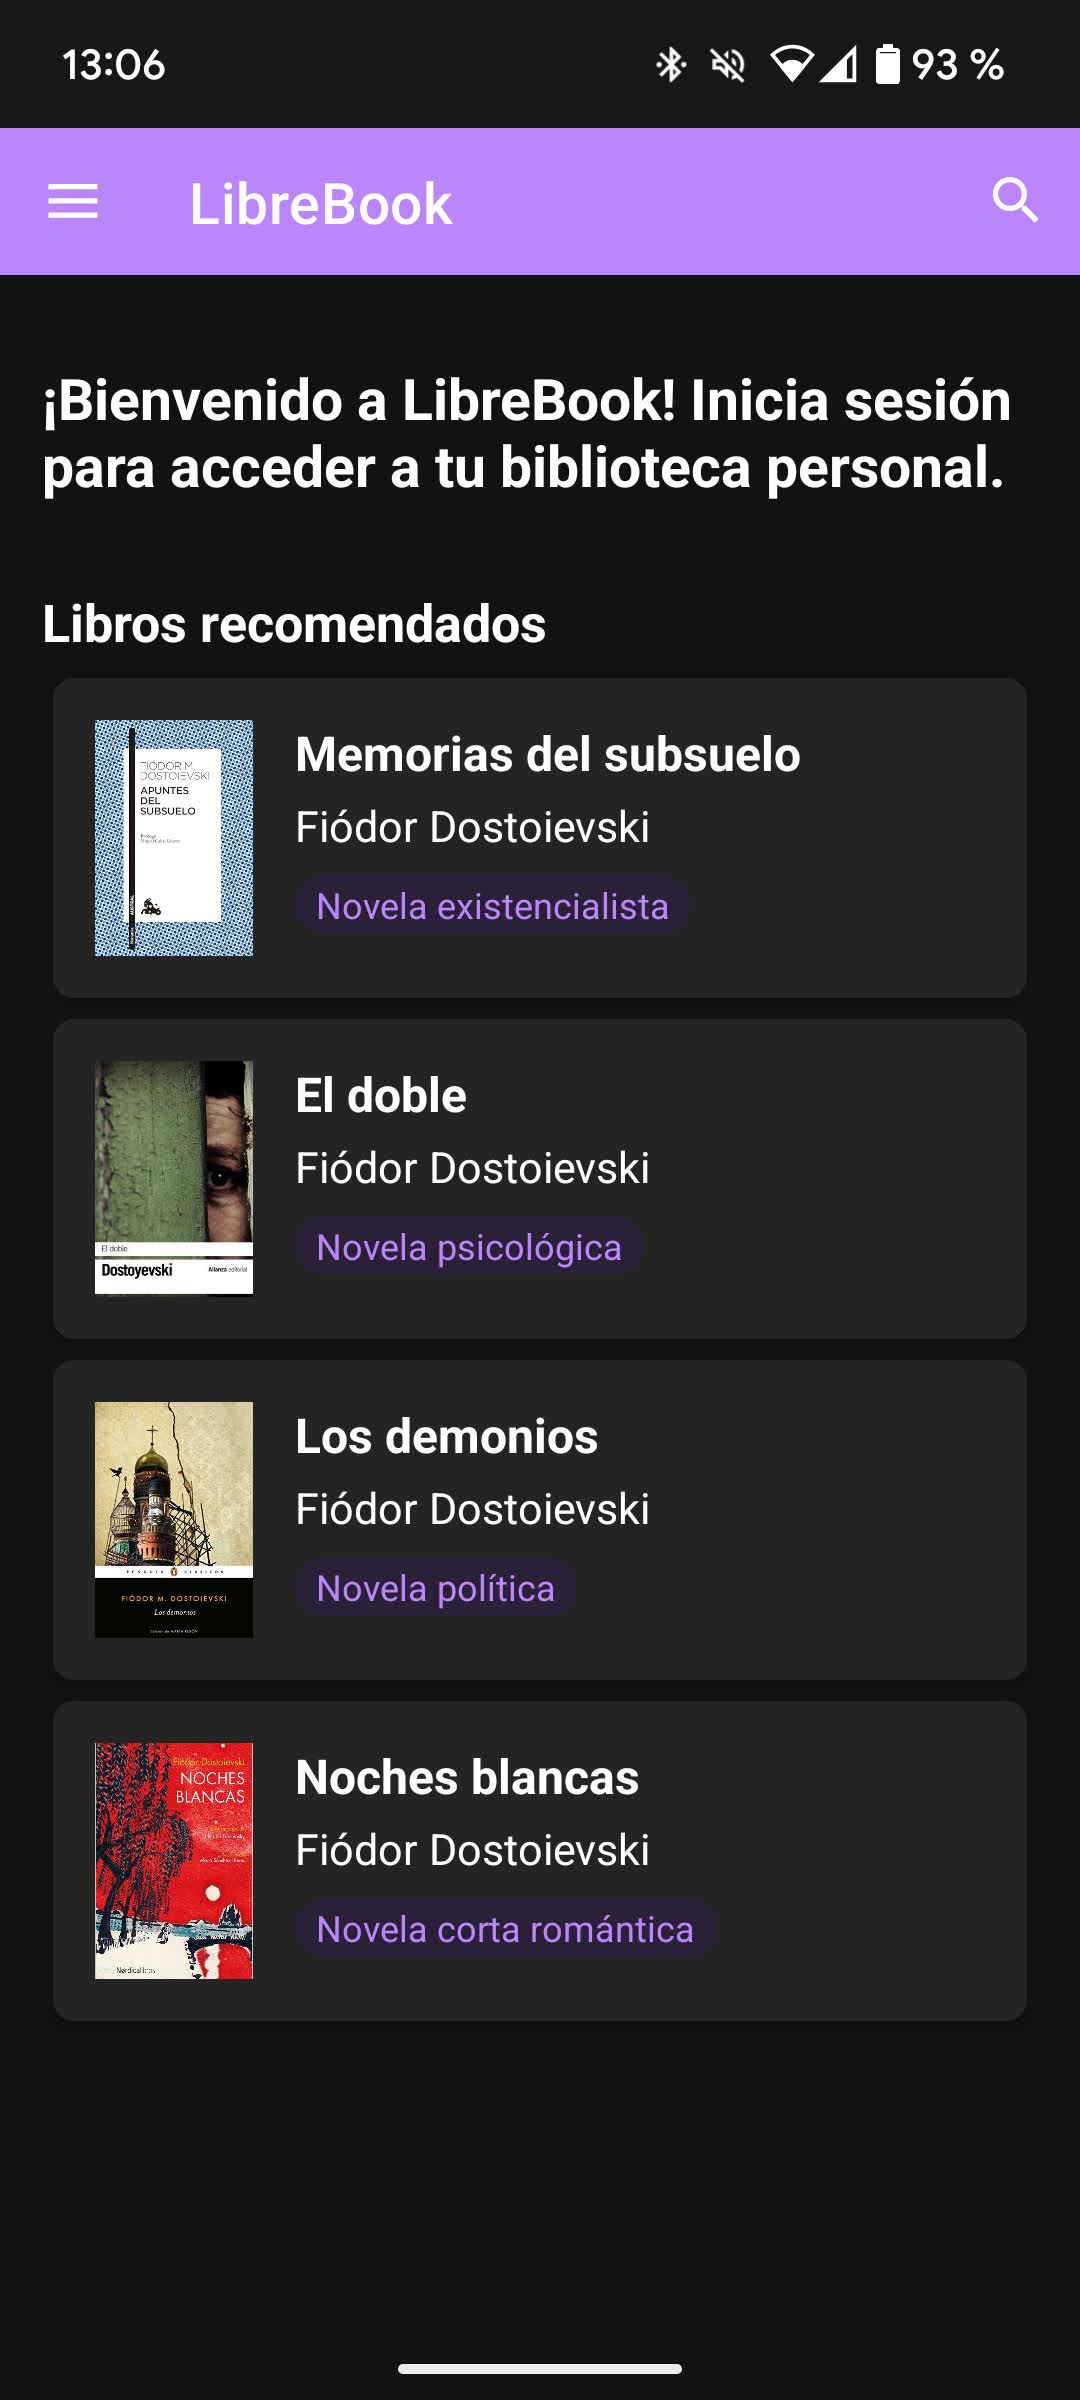
\includegraphics[width=0.95\linewidth]{.img/inicio.png}
          \caption{Pantalla de inicio}
        \end{figure}
        \vspace{-0.8em}  % Reduce espacio después de la figura
        
        \section{Menú de navegación}
        \vspace{-0.8em}  % Reduce espacio después del título
        El menú lateral permite acceder a todas las funciones de la aplicación. Las opciones varían según si has iniciado sesión o no.
        
        \begin{figure}[H]
          \centering
          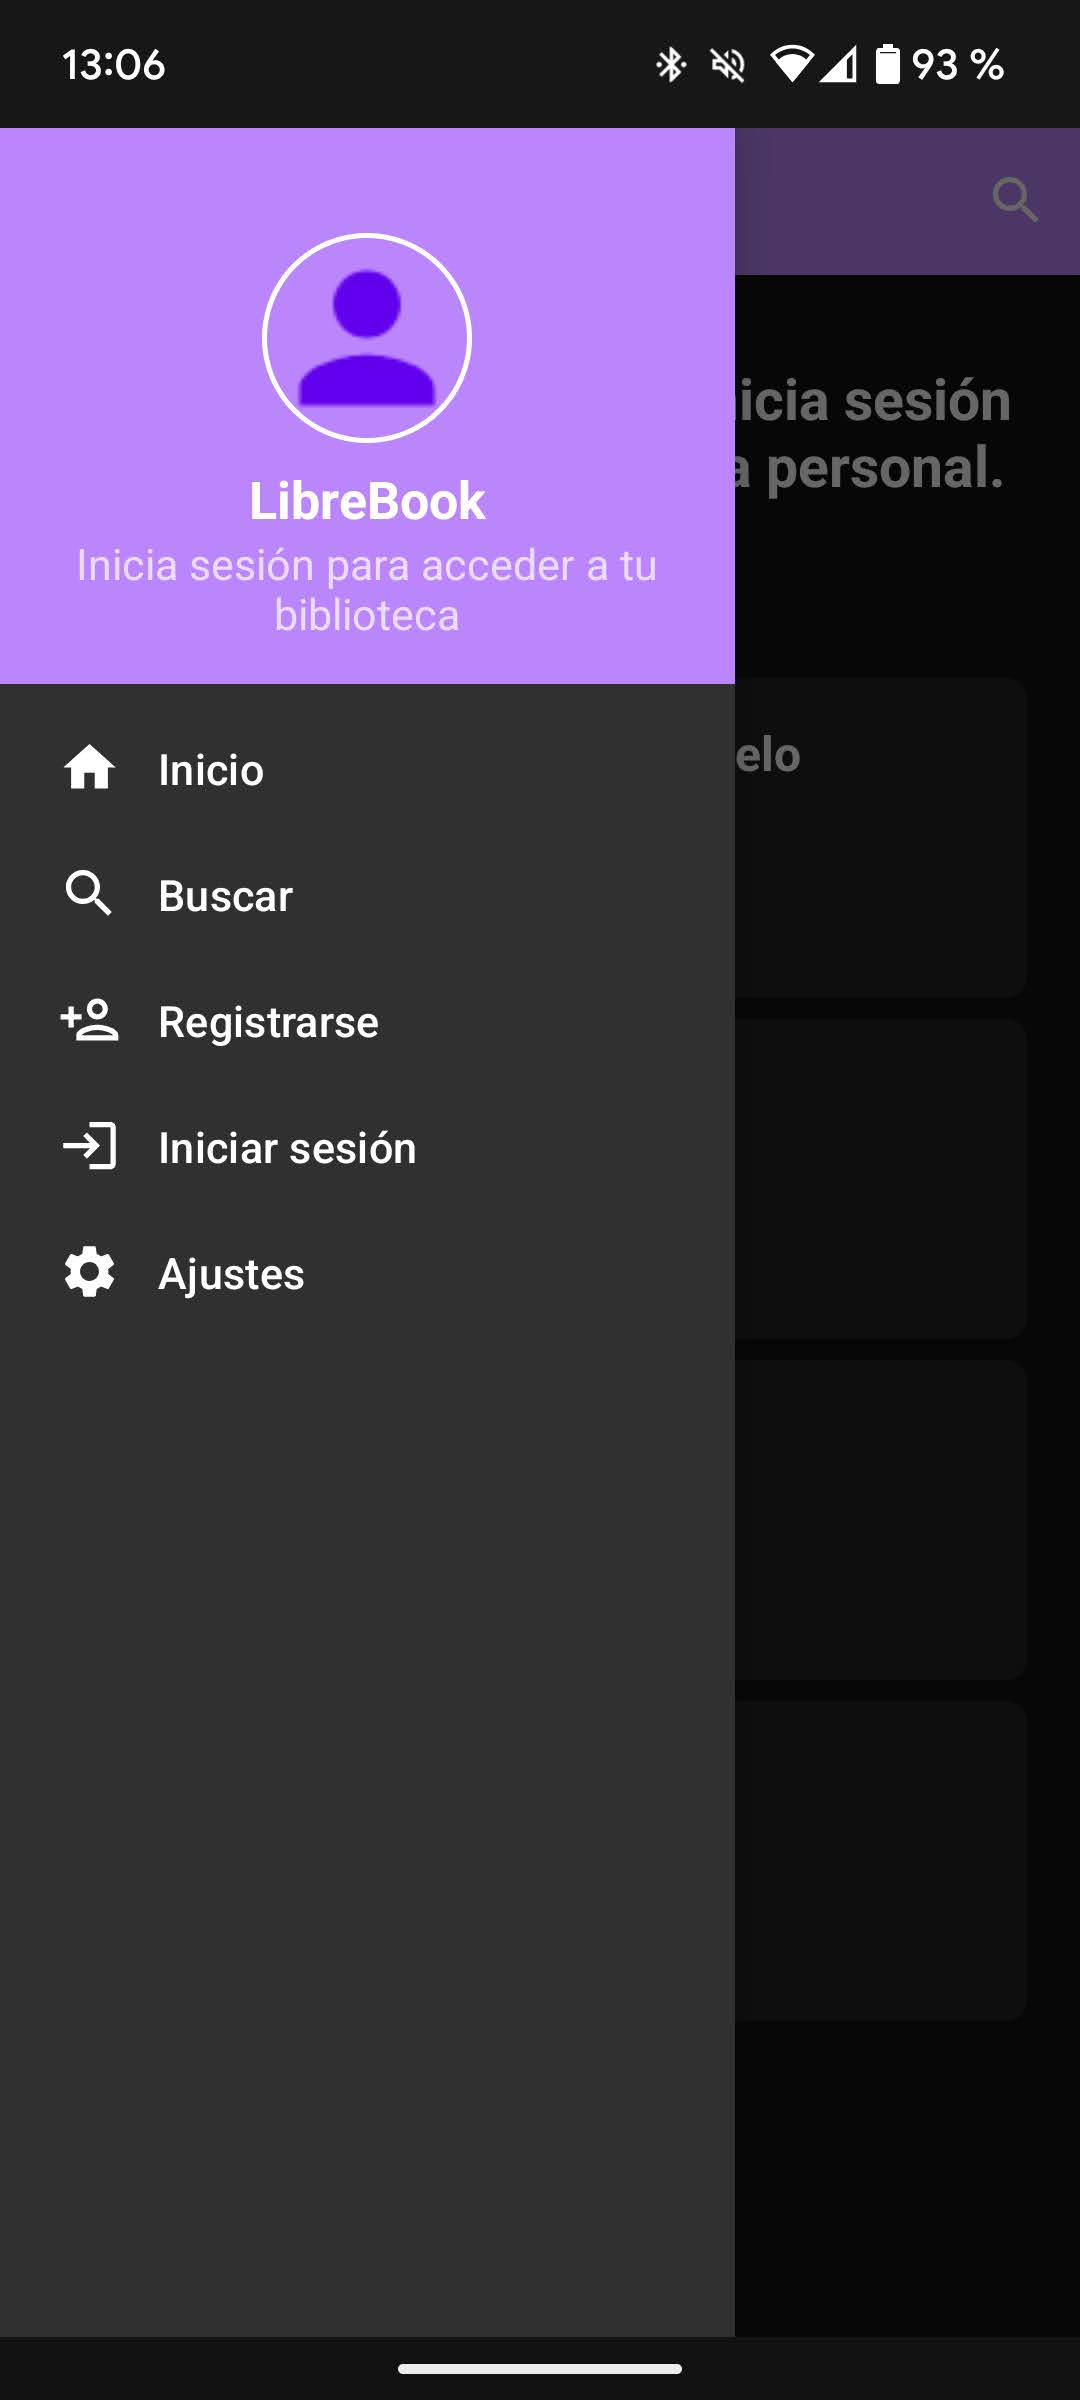
\includegraphics[width=0.47\linewidth]{.img/menu.png}\hfill
          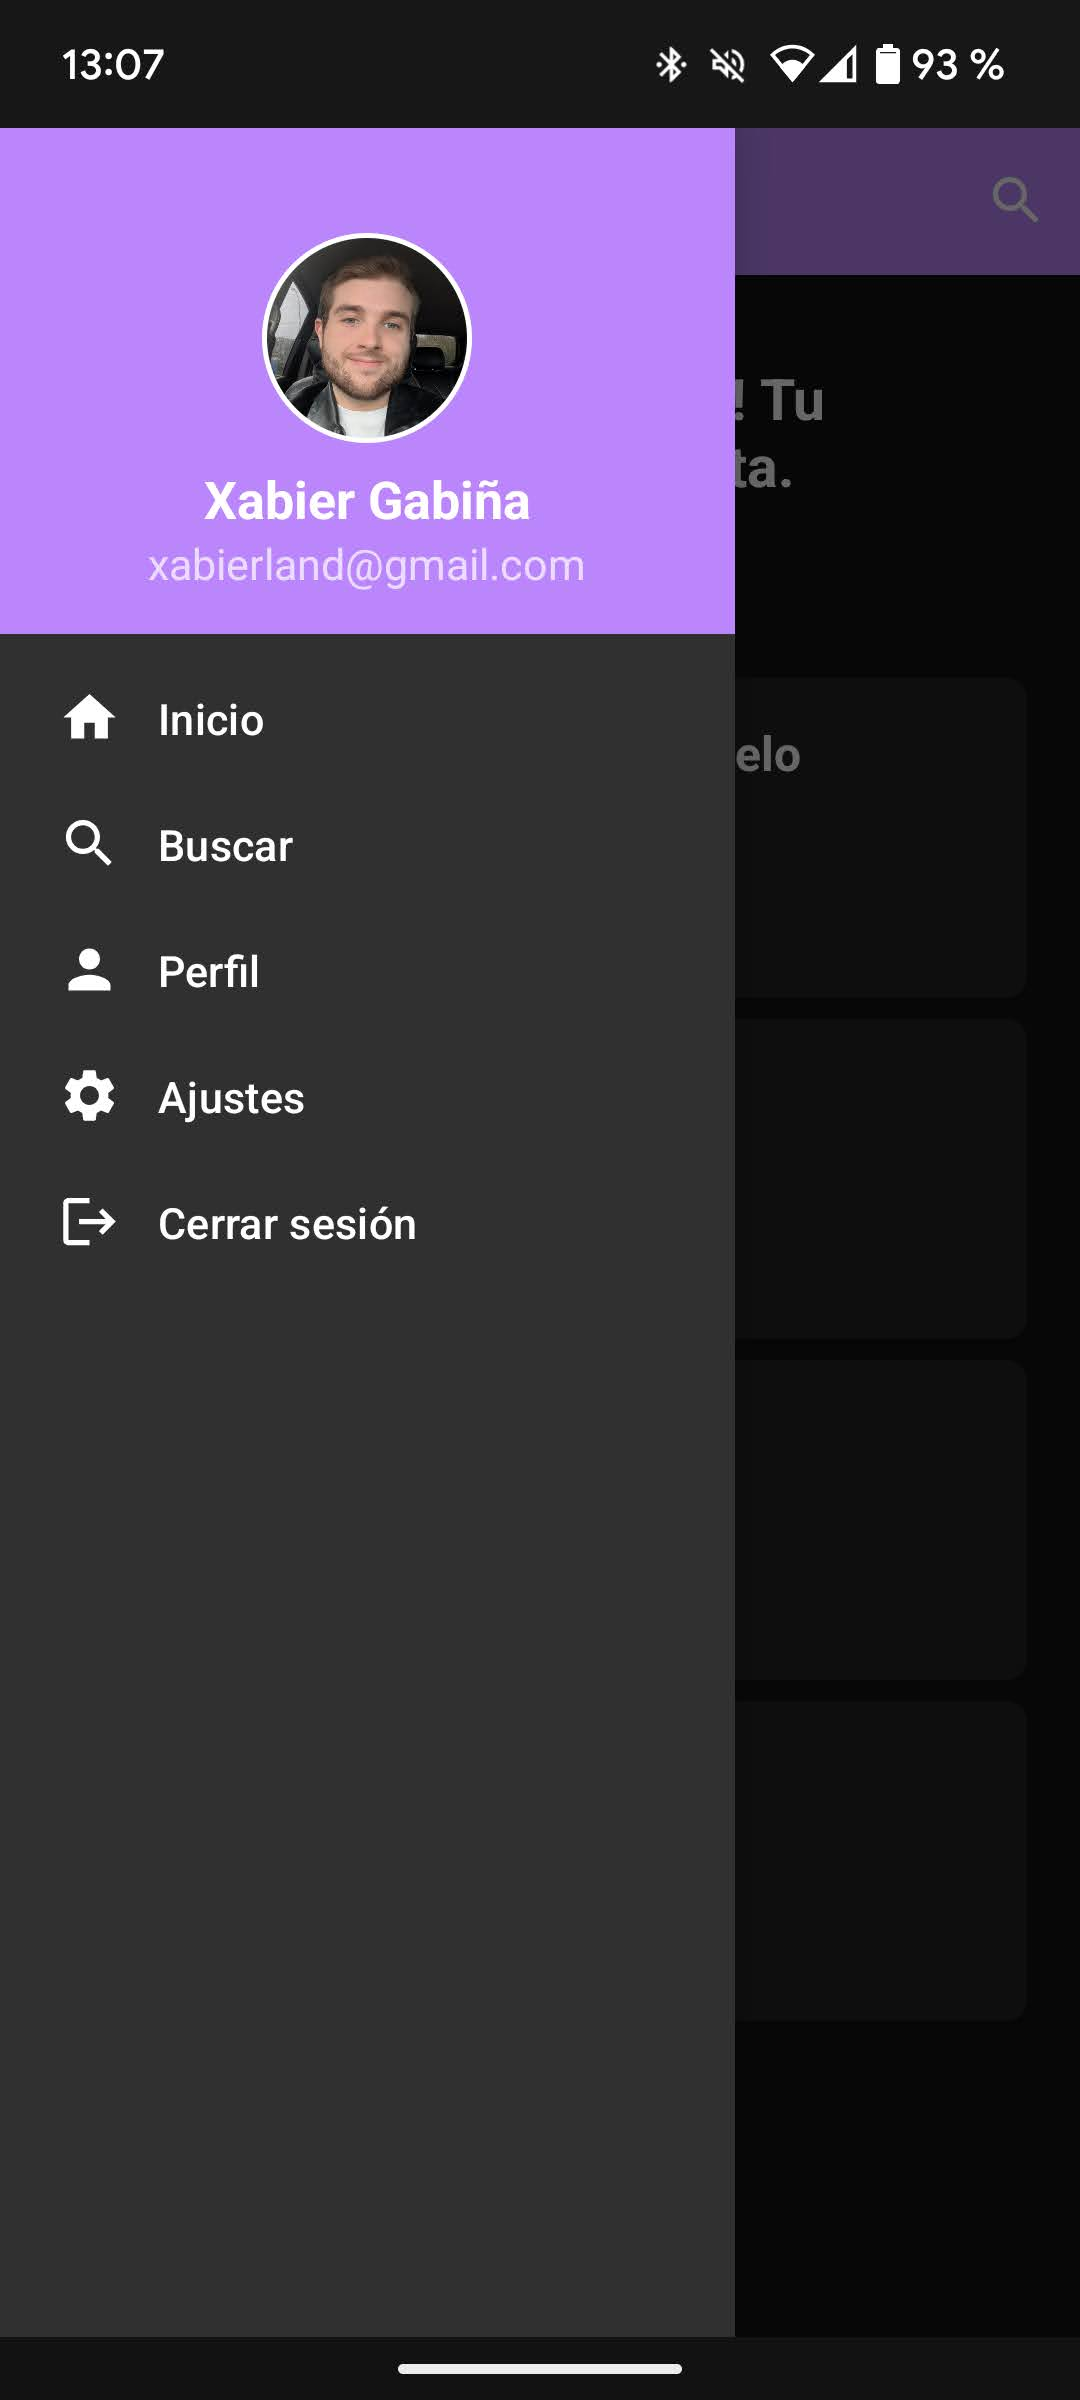
\includegraphics[width=0.47\linewidth]{.img/menu-auth.png}
          \caption{Menú para usuario anónimo (izq.) y autenticado (der.)}
        \end{figure}
        \vspace{-0.8em}  % Reduce espacio después de la figura
        
        \section{Registrarse e iniciar sesión}
        \vspace{-0.8em}  % Reduce espacio después del título
        Para acceder a toda la funcionalidad, necesitas crear una cuenta o iniciar sesión con credenciales existentes.
        
        \begin{figure}[H]
          \centering
          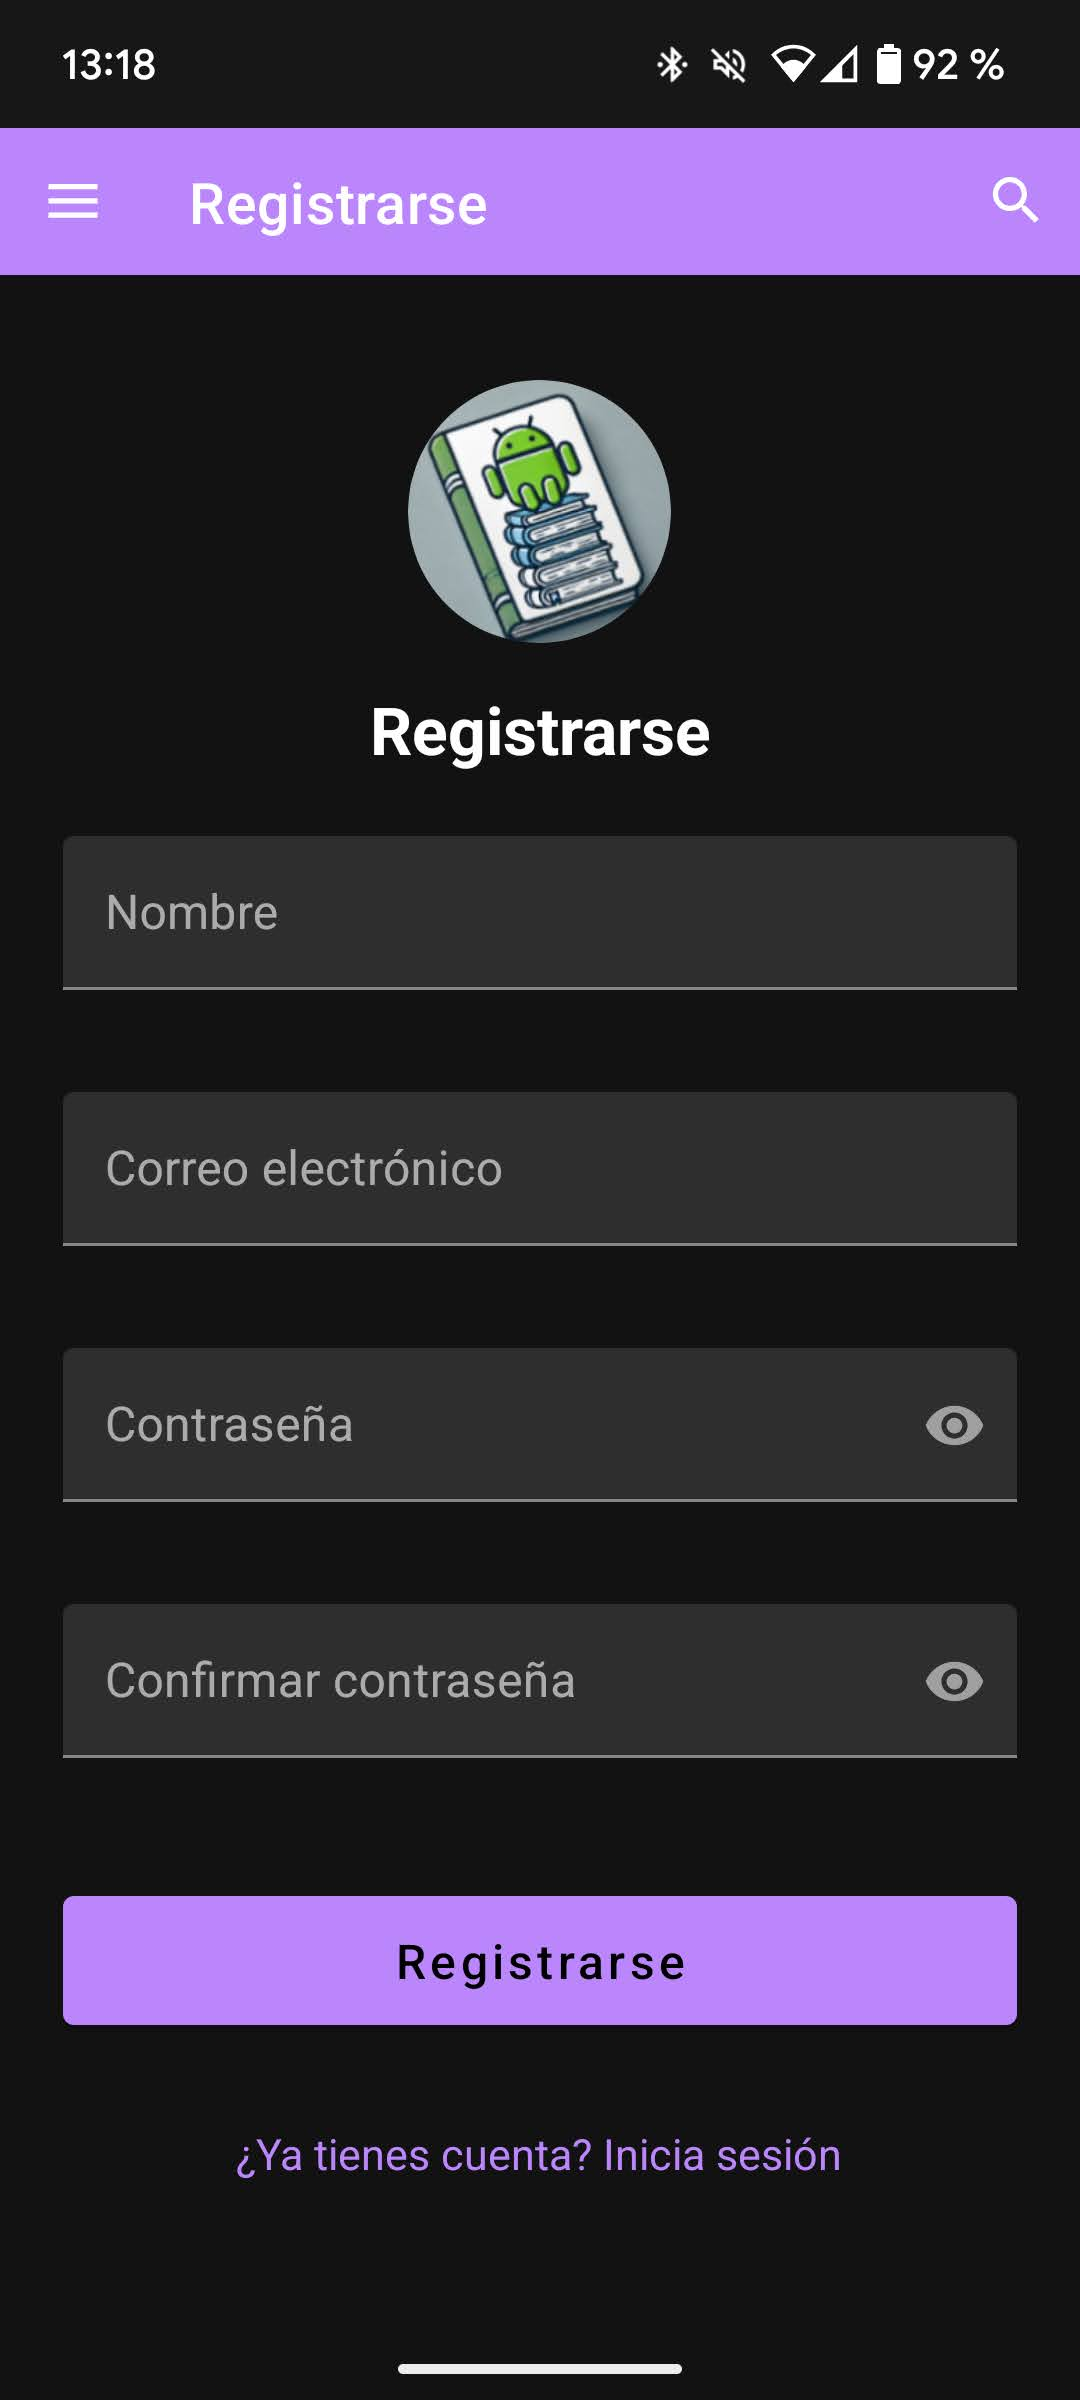
\includegraphics[width=0.47\linewidth]{.img/registro.png}\hfill
          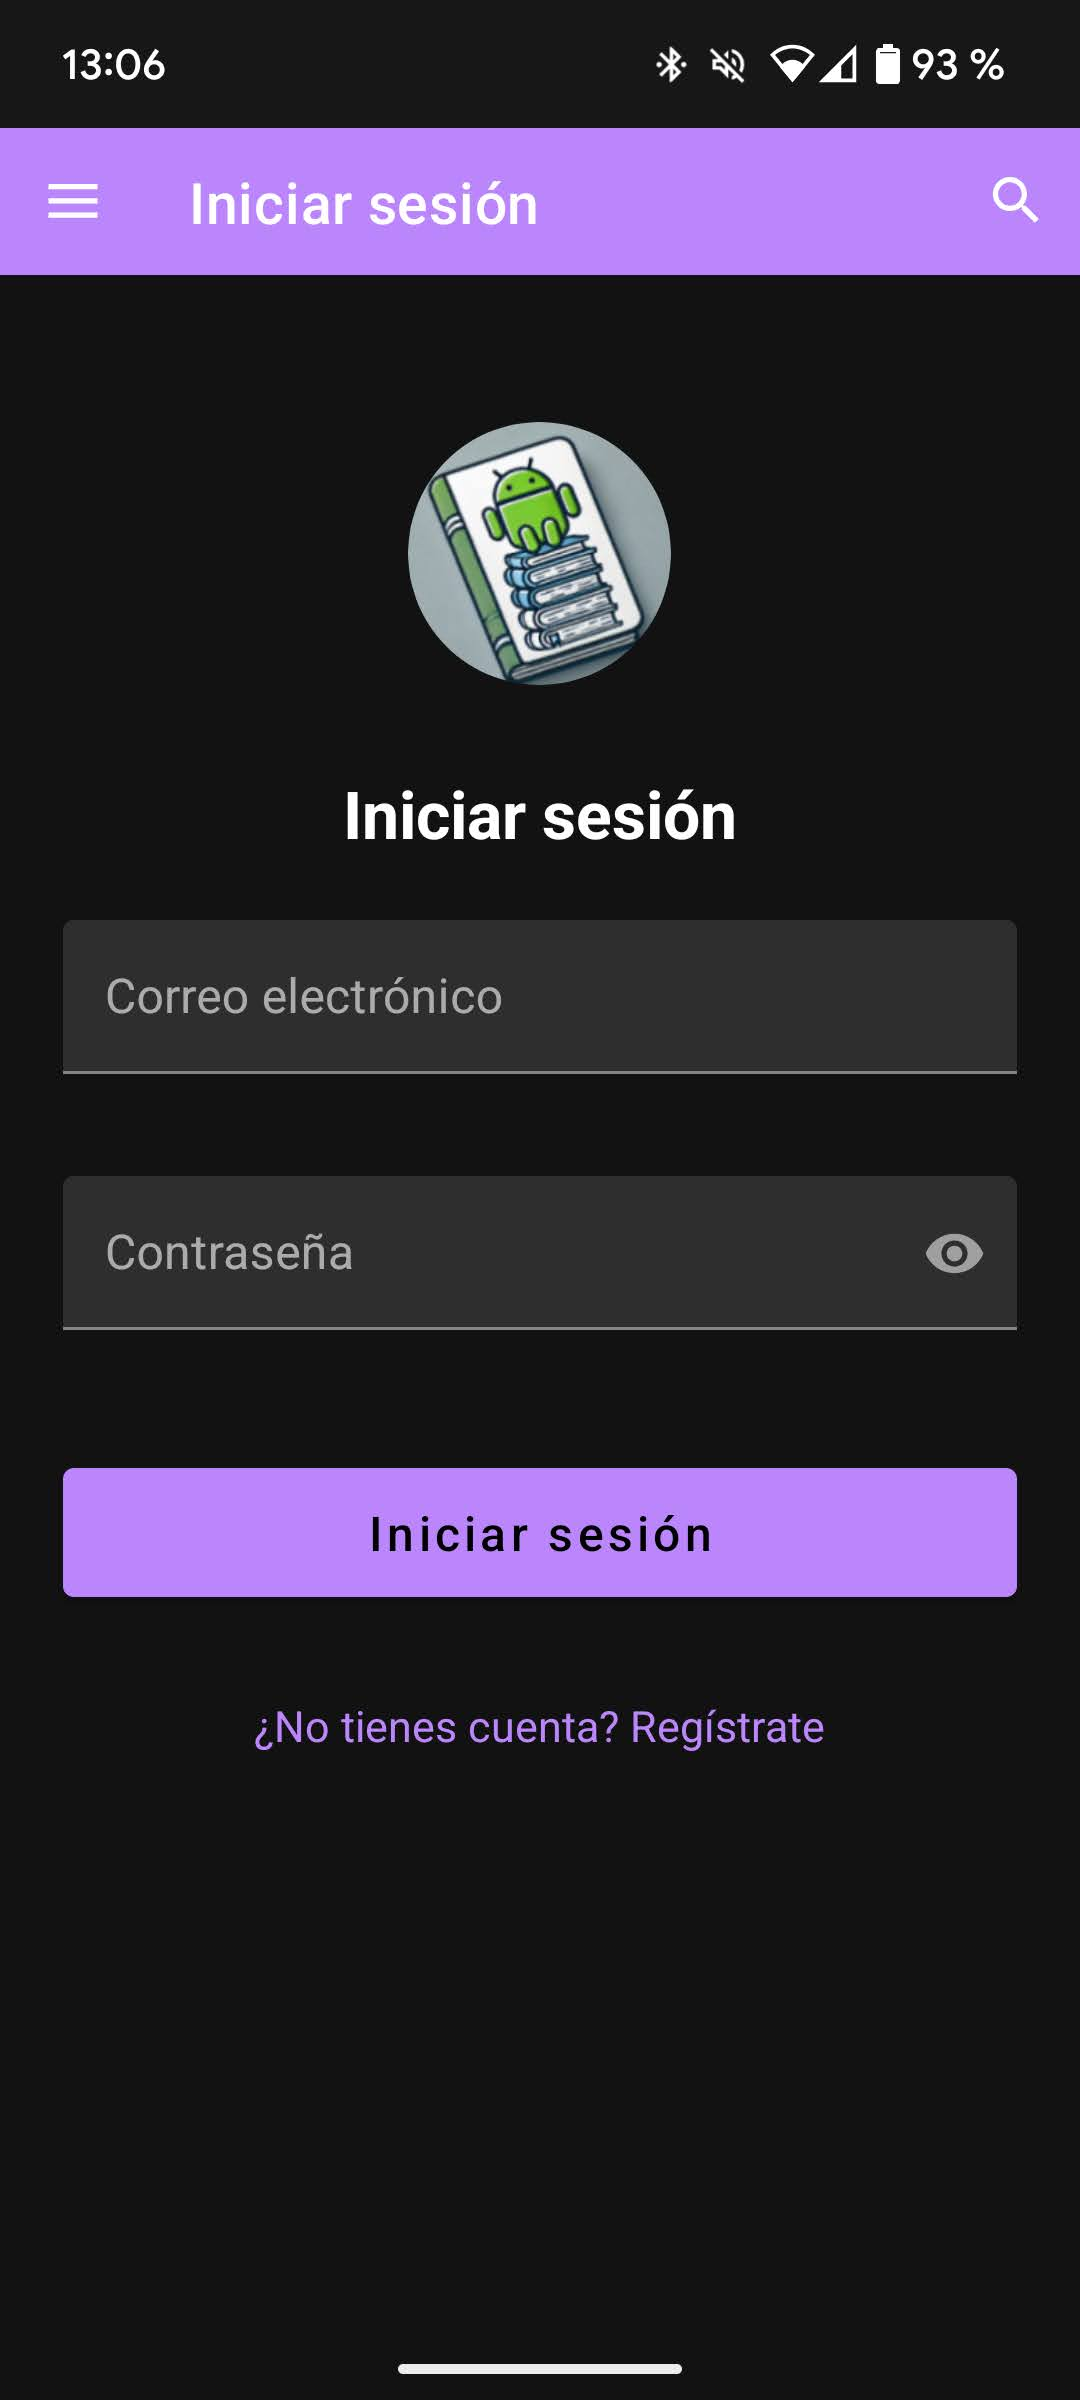
\includegraphics[width=0.47\linewidth]{.img/login.png}
          \caption{Pantallas de registro (izq.) e inicio de sesión (der.)}
        \end{figure}
        
        Al registrarte, recibirás una notificación de bienvenida.
        
        \begin{figure}[H]
          \centering
          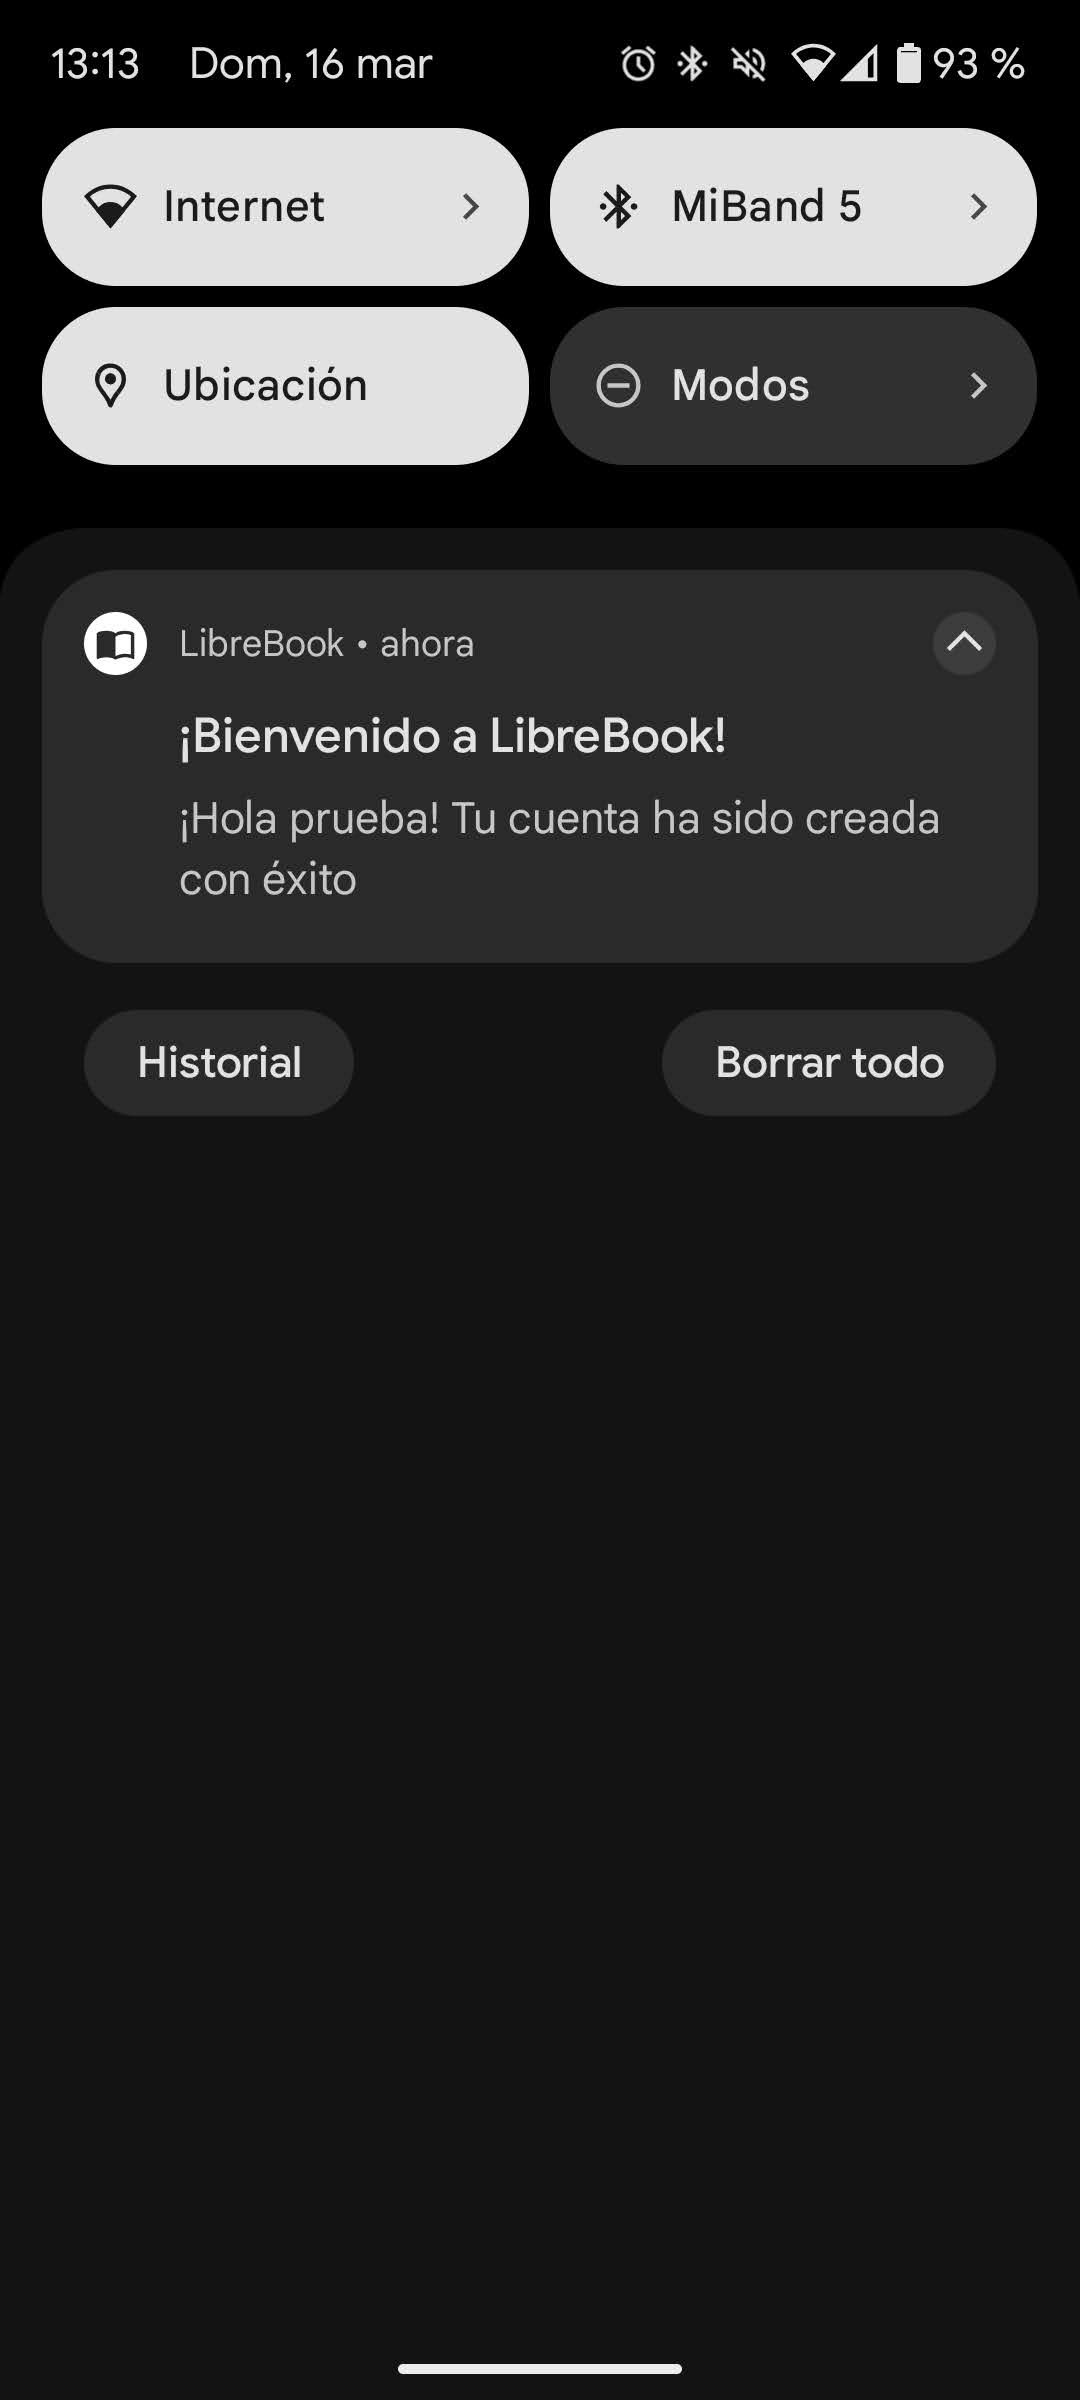
\includegraphics[width=0.65\linewidth]{.img/registro-noti.png}
          \caption{Notificación de bienvenida}
        \end{figure}
        \vspace{-0.8em}  % Reduce espacio después de la figura
        
        \section{Ver tu biblioteca}
        \vspace{-0.8em}  % Reduce espacio después del título
        Tu perfil muestra tus estadísticas de lectura y tus libros organizados en tres categorías: Leyendo, Por leer y Leídos.
        
        \begin{figure}[H]
          \centering
          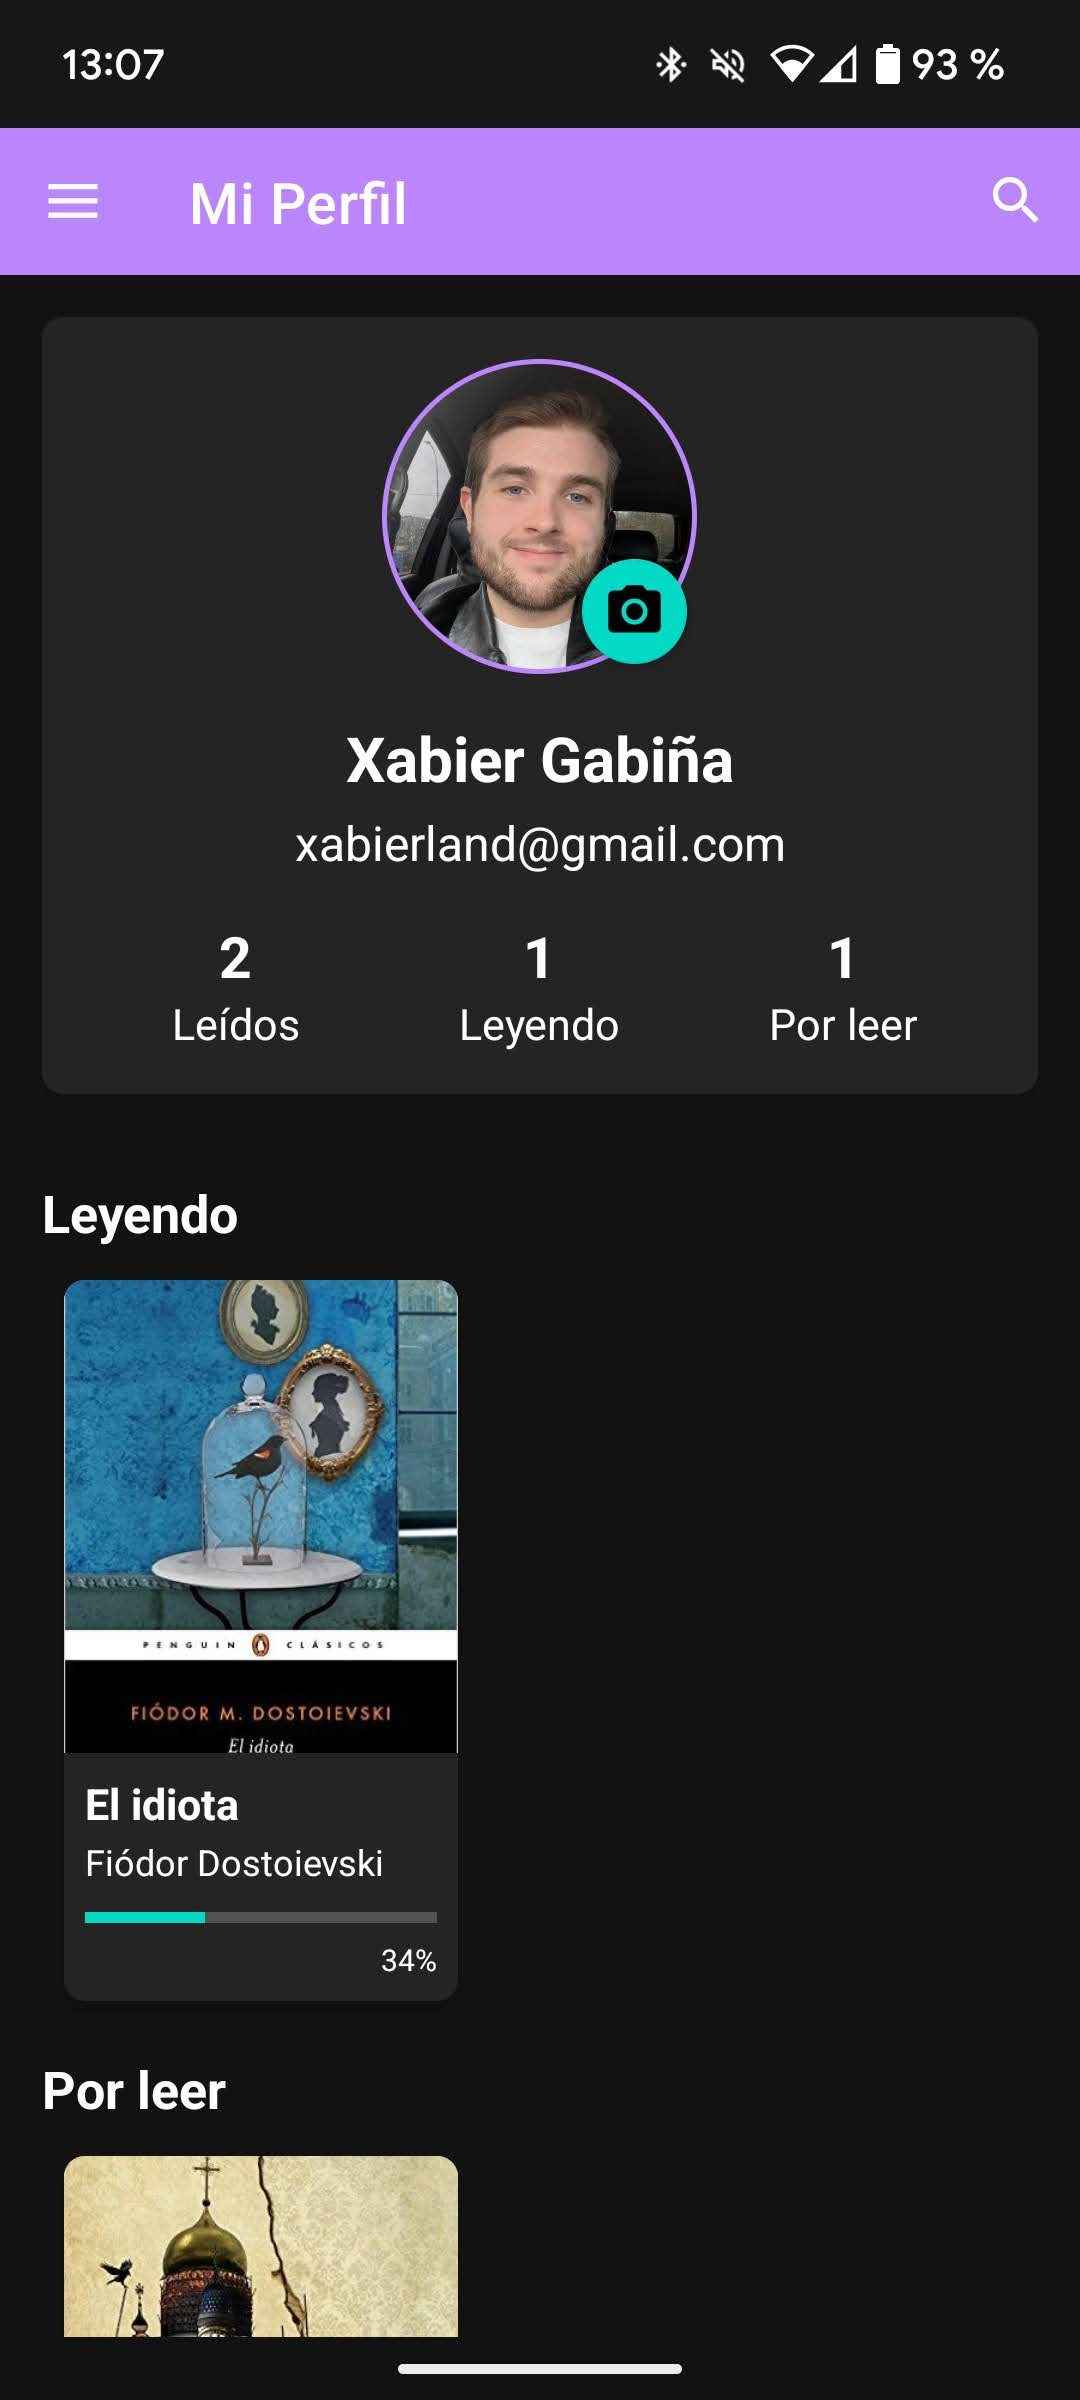
\includegraphics[width=0.95\linewidth]{.img/profile.png}
          \caption{Perfil del usuario}
        \end{figure}
        
        Puedes cambiar tu foto de perfil pulsando el icono de cámara, para lo cual la aplicación solicitará permisos.
        
        \columnbreak
        
        \section{Buscar libros o usuarios}
        \vspace{-0.8em}  % Reduce espacio después del título
        La función de búsqueda permite encontrar libros por título o autor, así como otros usuarios.
        
        \begin{figure}[H]
          \centering
          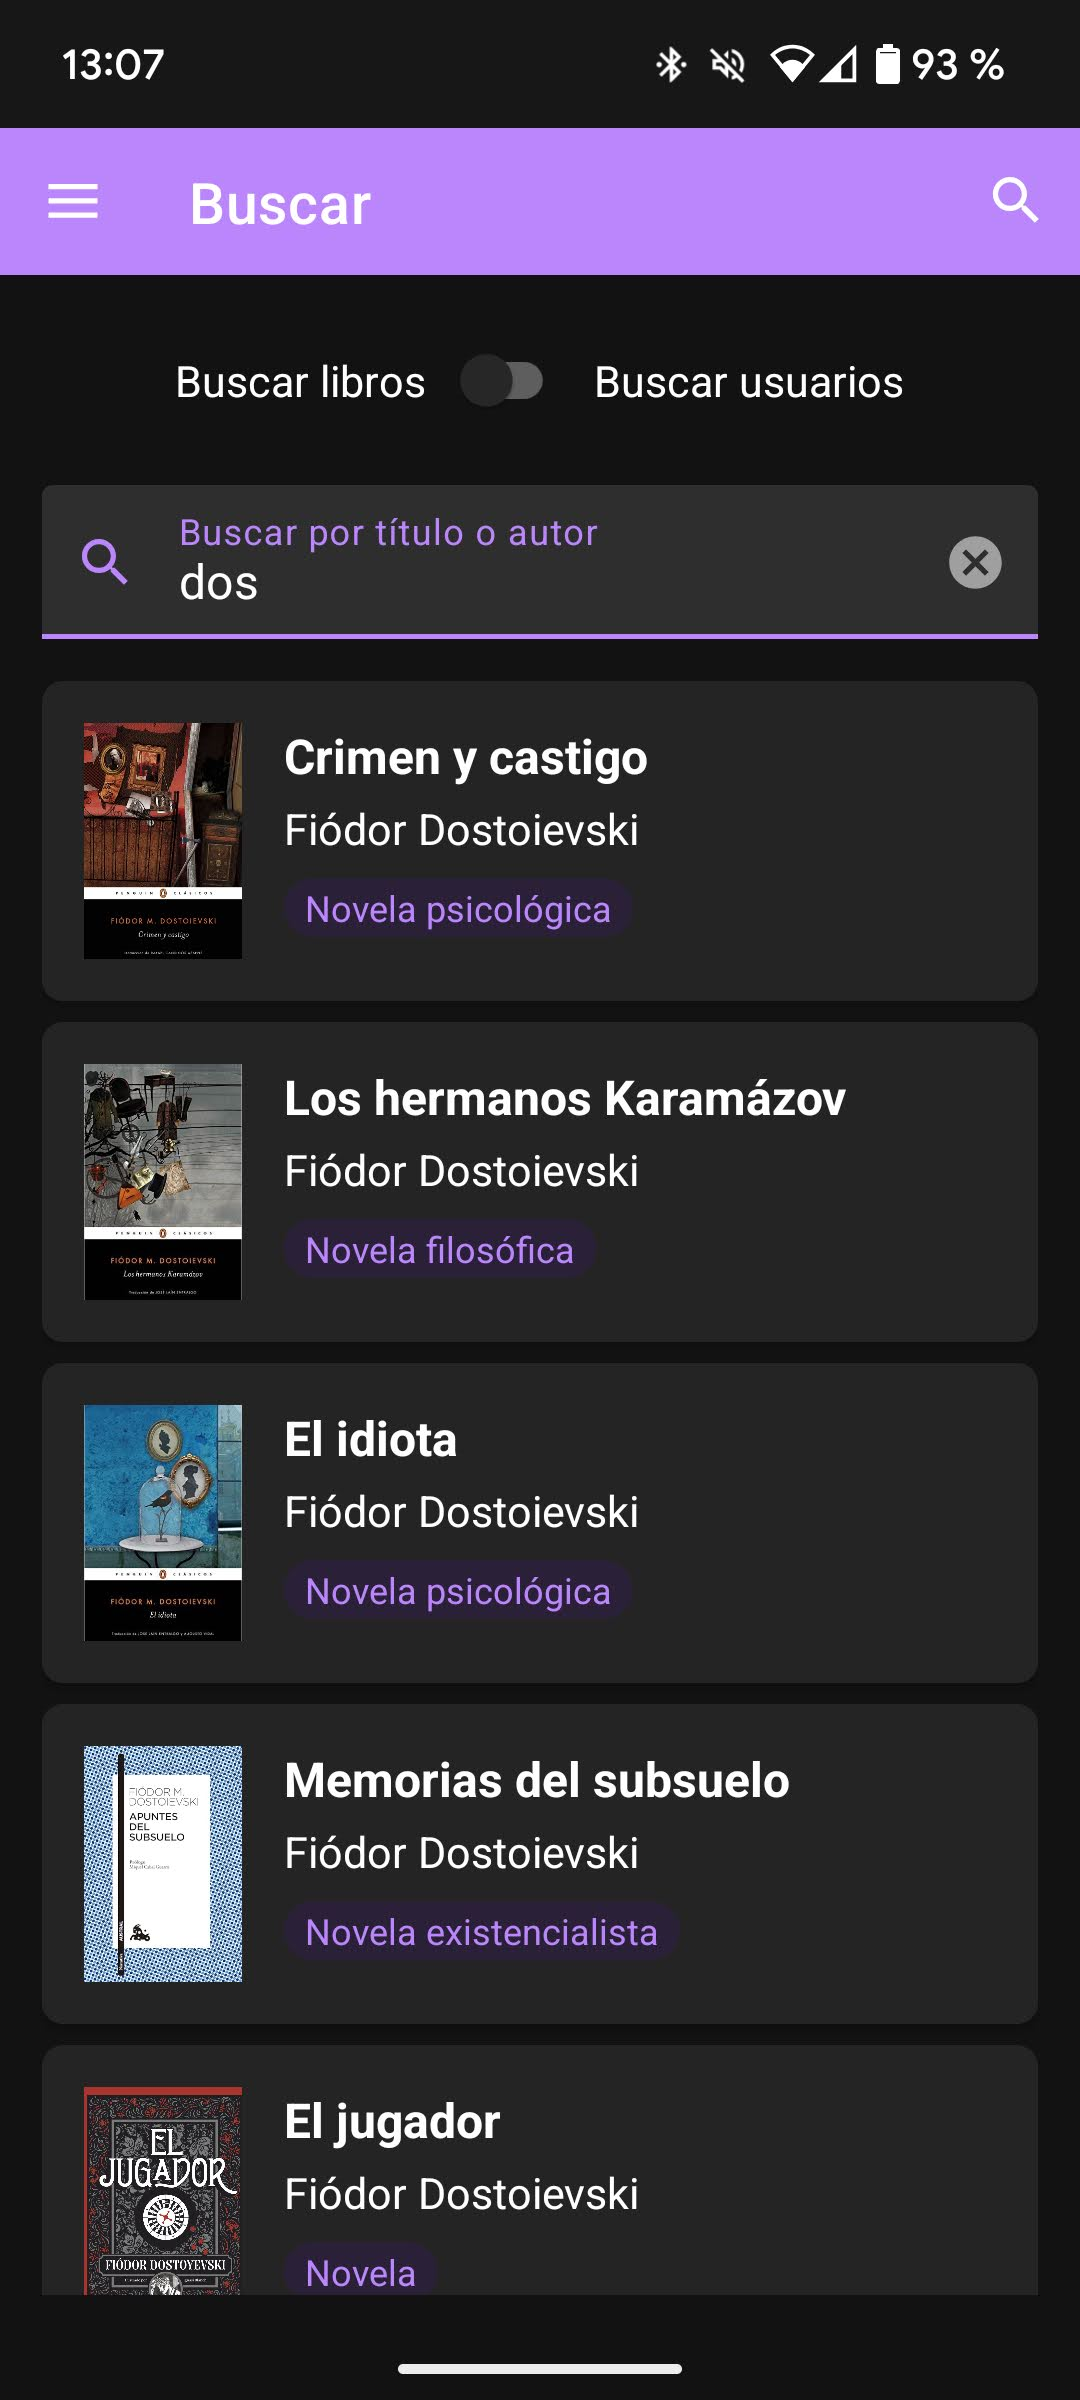
\includegraphics[width=0.47\linewidth]{.img/buscador-libros.png}\hfill
          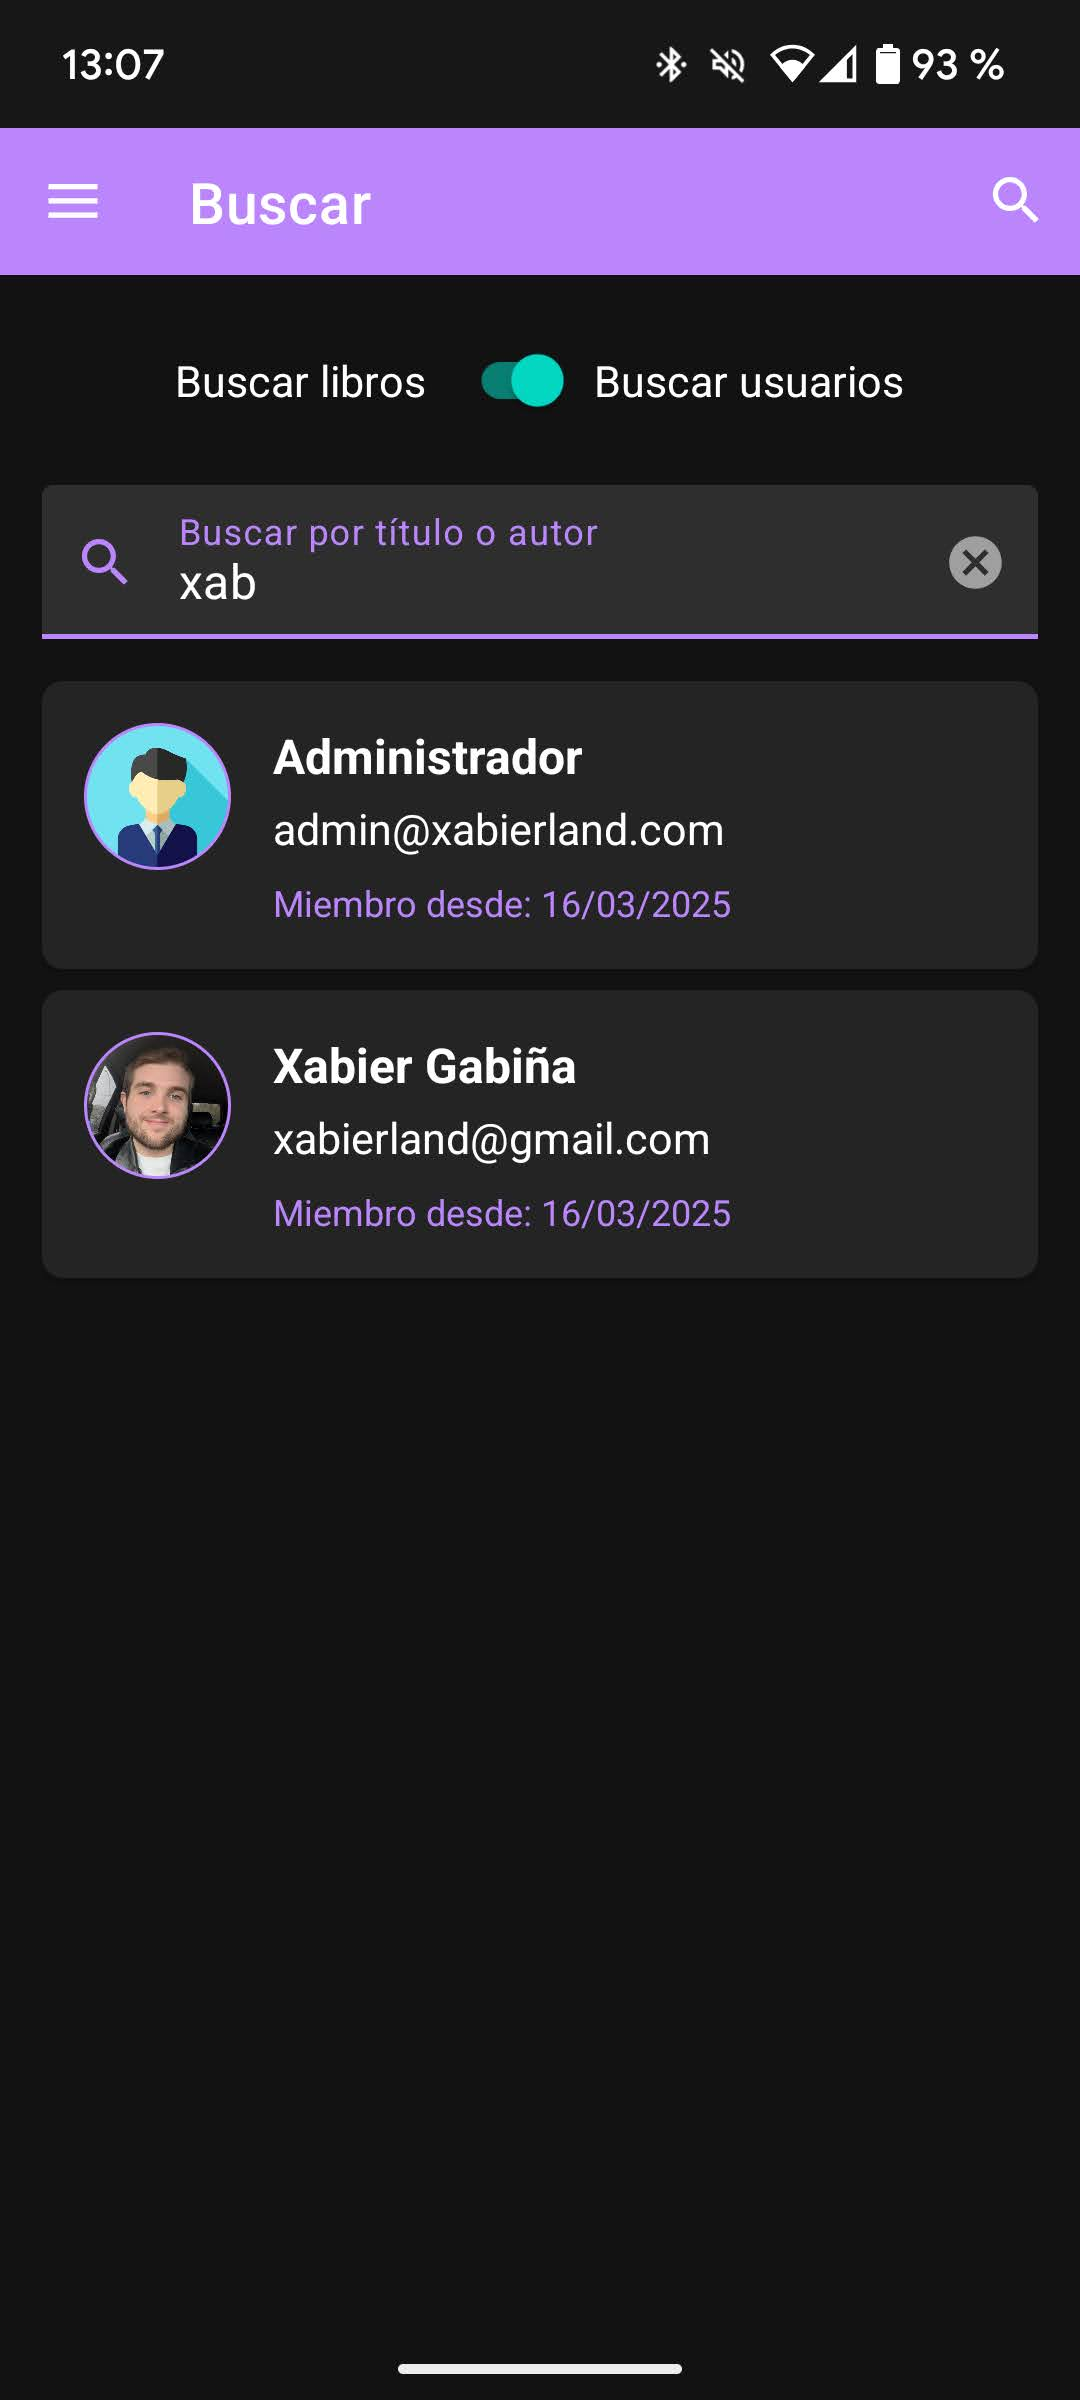
\includegraphics[width=0.47\linewidth]{.img/buscador-usuarios.png}
          \caption{Búsqueda de libros (izq.) y usuarios (der.)}
        \end{figure}
        \vspace{-0.8em}  % Reduce espacio después de la figura
        
        \section{Añadir libros a tu biblioteca}
        \vspace{-0.8em}  % Reduce espacio después del título
        Al encontrar un libro, puedes ver sus detalles y añadirlo a tu biblioteca en diferentes estados.
        
        \begin{figure}[H]
          \centering
          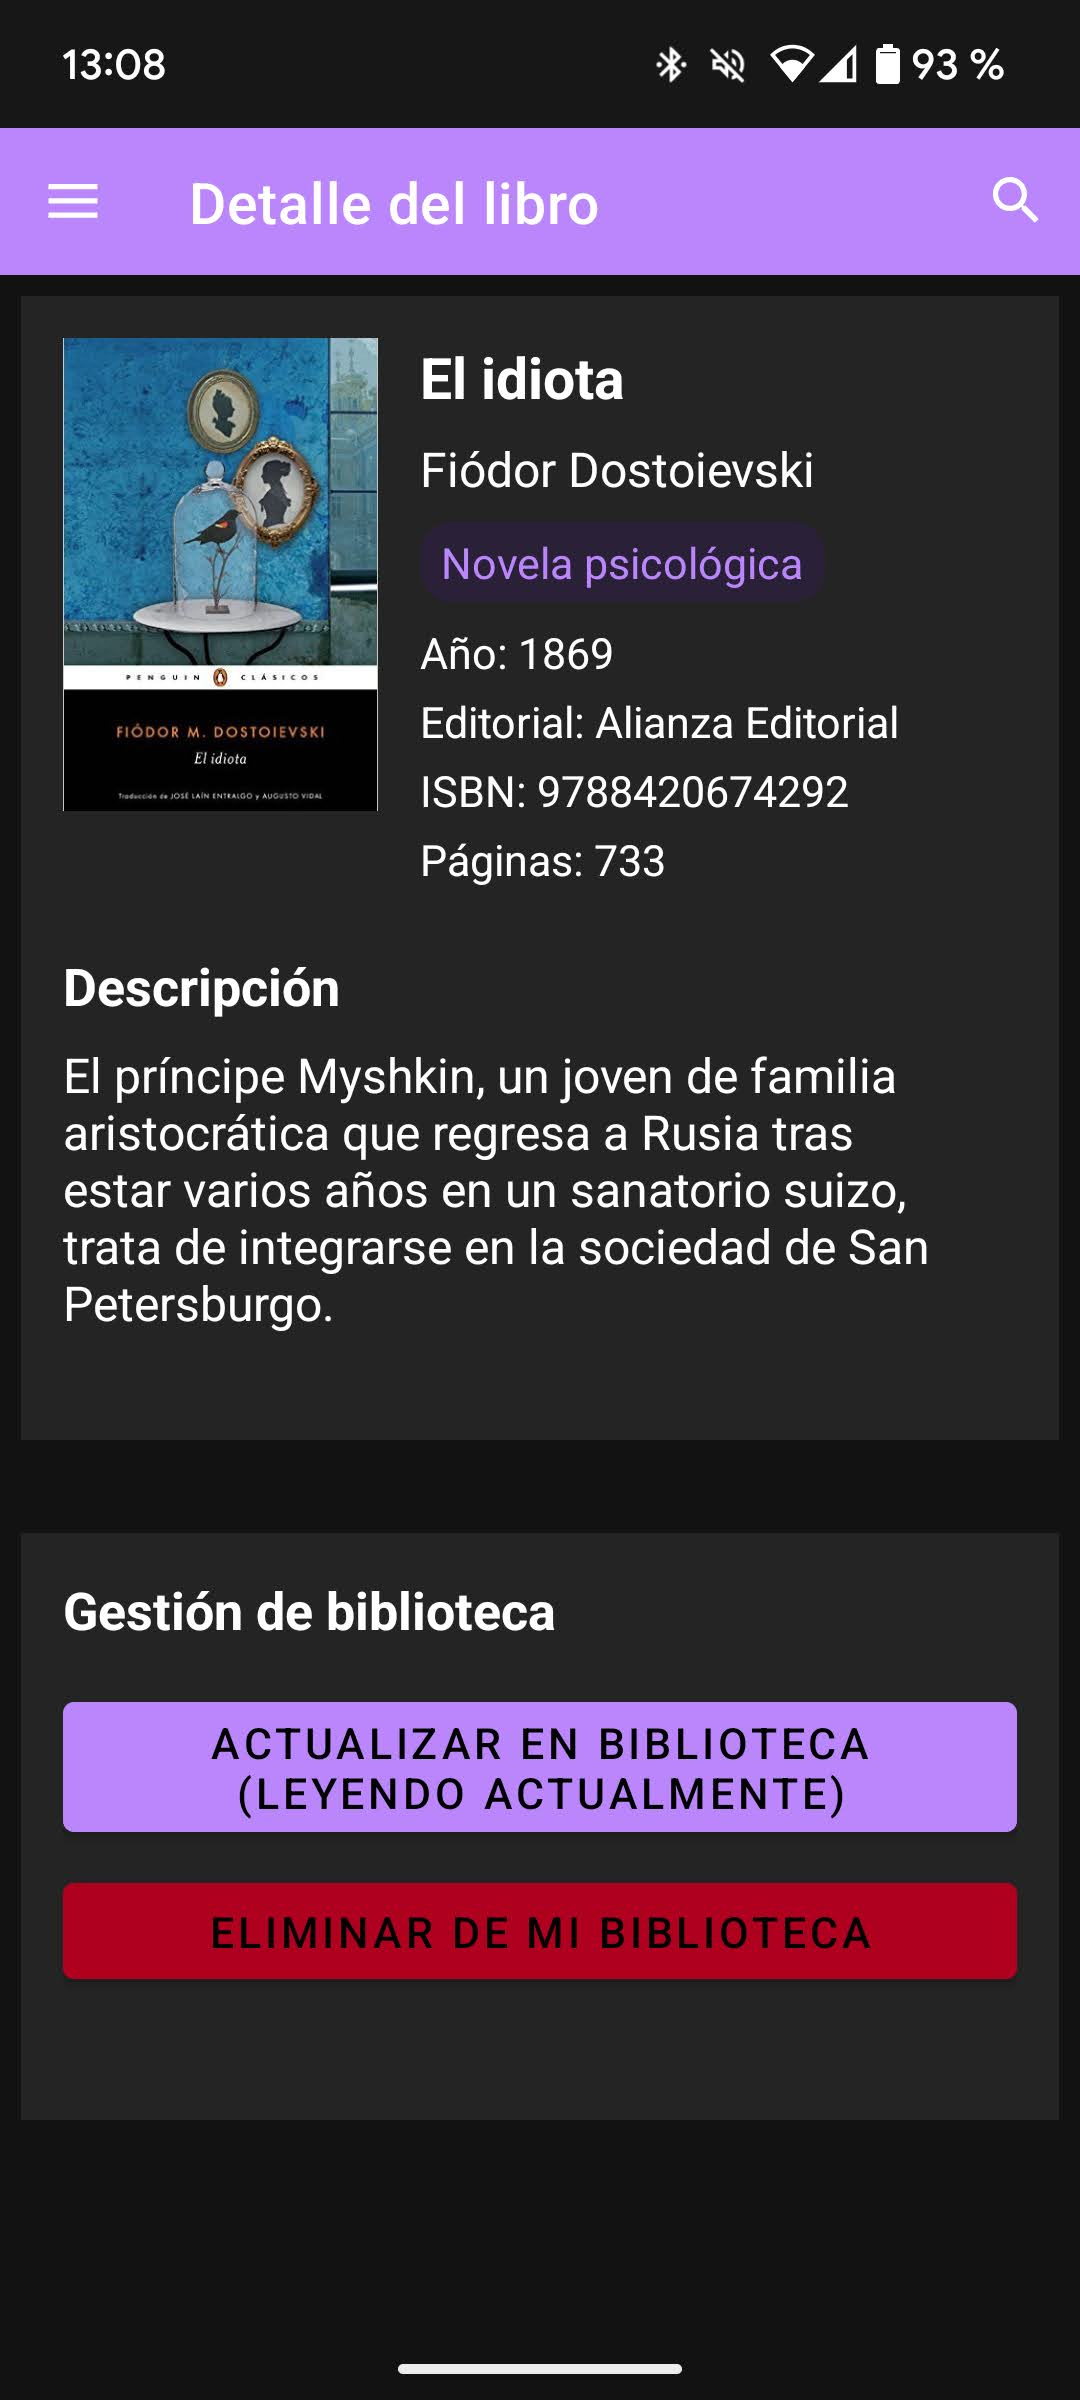
\includegraphics[width=0.95\linewidth]{.img/libro.png}
          \caption{Pantalla de detalle de libro}
        \end{figure}
        
        \begin{figure}[H]
          \centering
          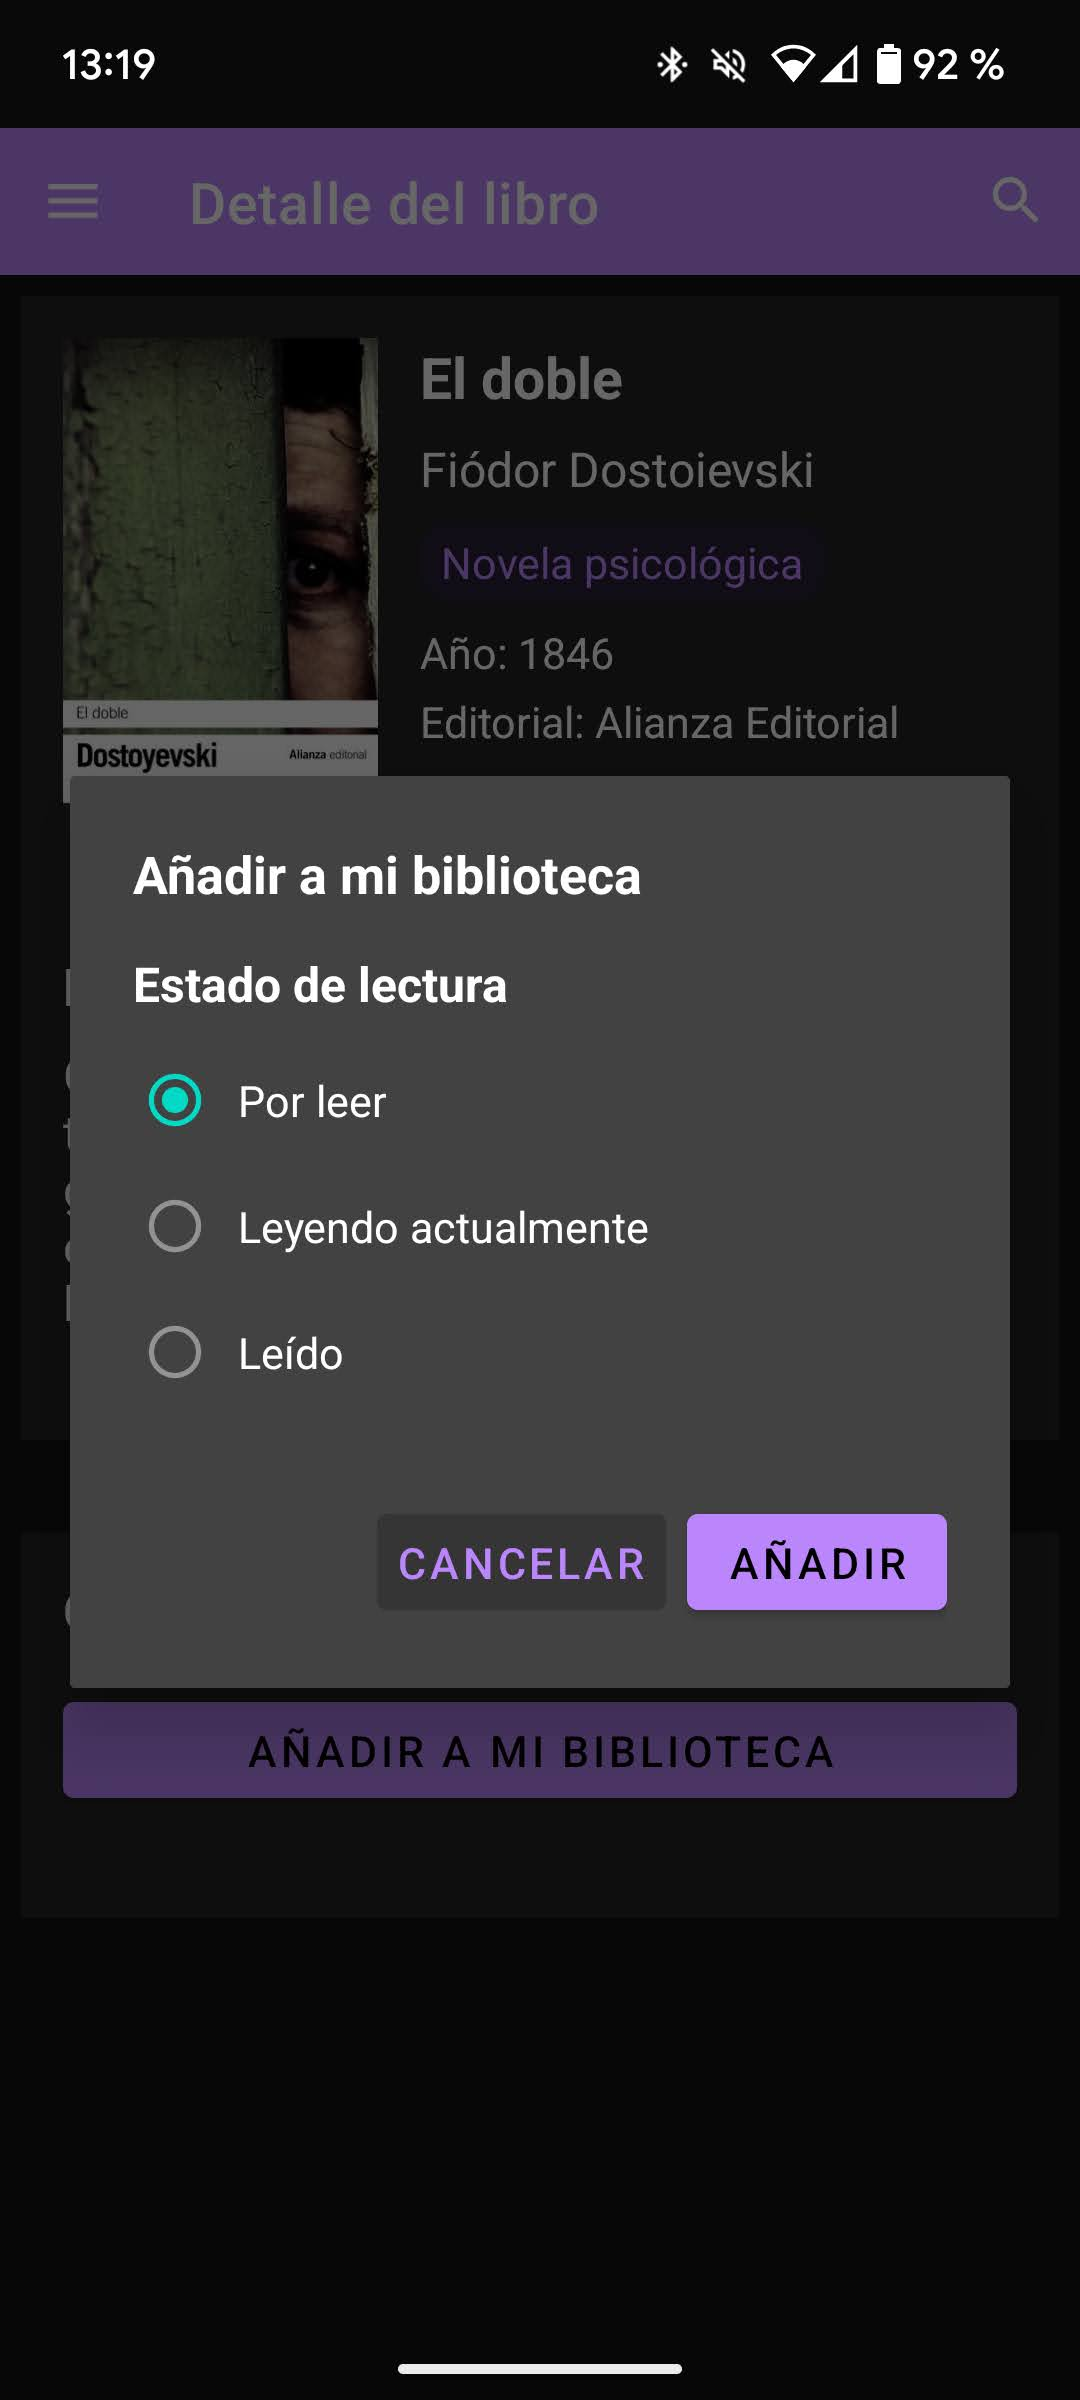
\includegraphics[width=0.47\linewidth]{.img/libro-porleer.png}\hfill
          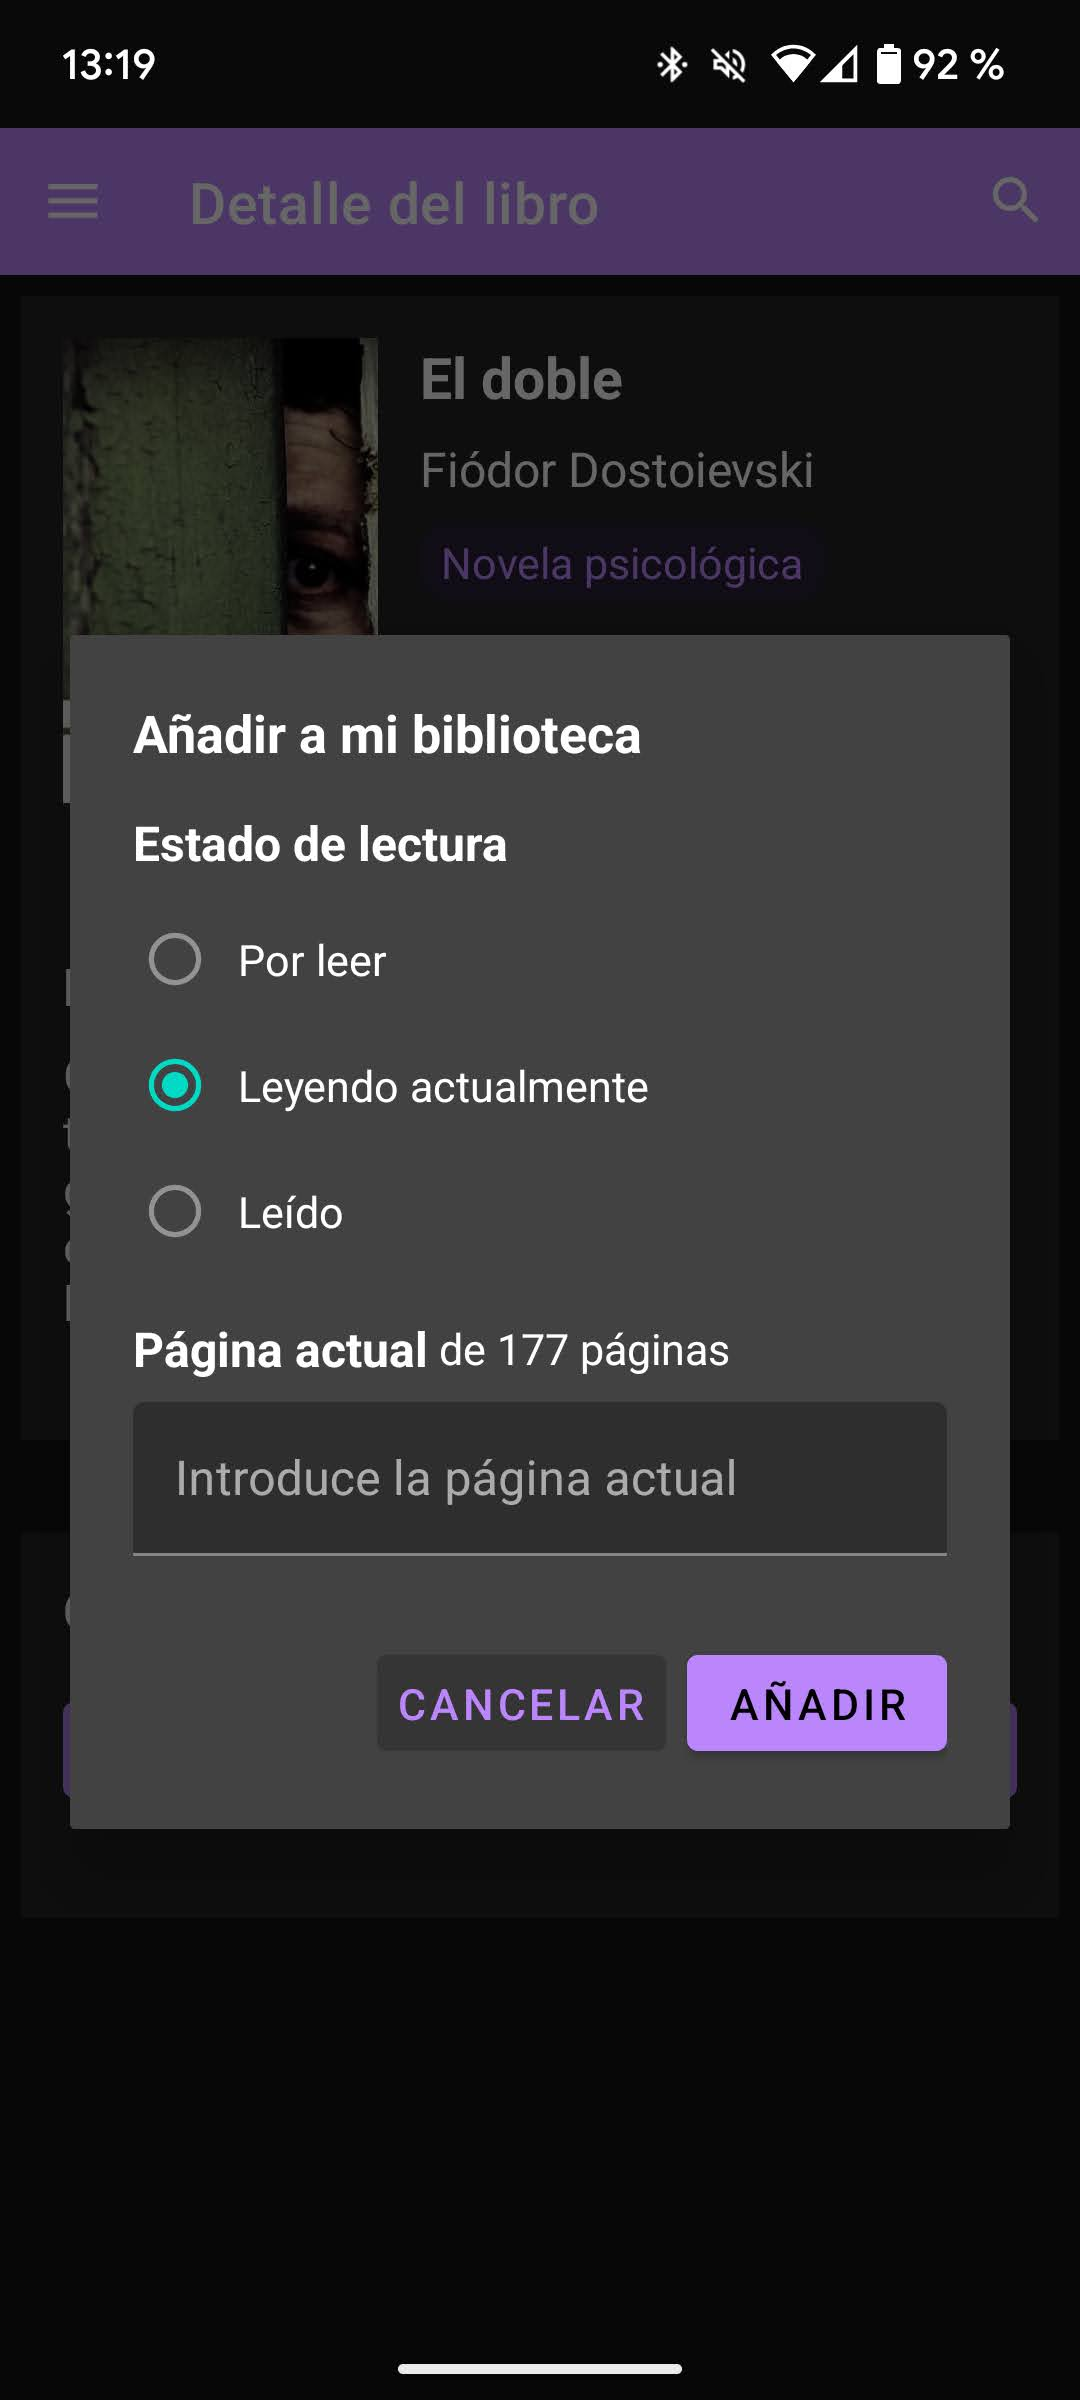
\includegraphics[width=0.47\linewidth]{.img/libro-leyendo.png}
          \caption{Añadir libro como "Por leer" (izq.) o "Leyendo" (der.)}
        \end{figure}
        
        Al añadir un libro como "Leído", puedes incluir una calificación y reseña.
        
        \begin{figure}[H]
          \centering
          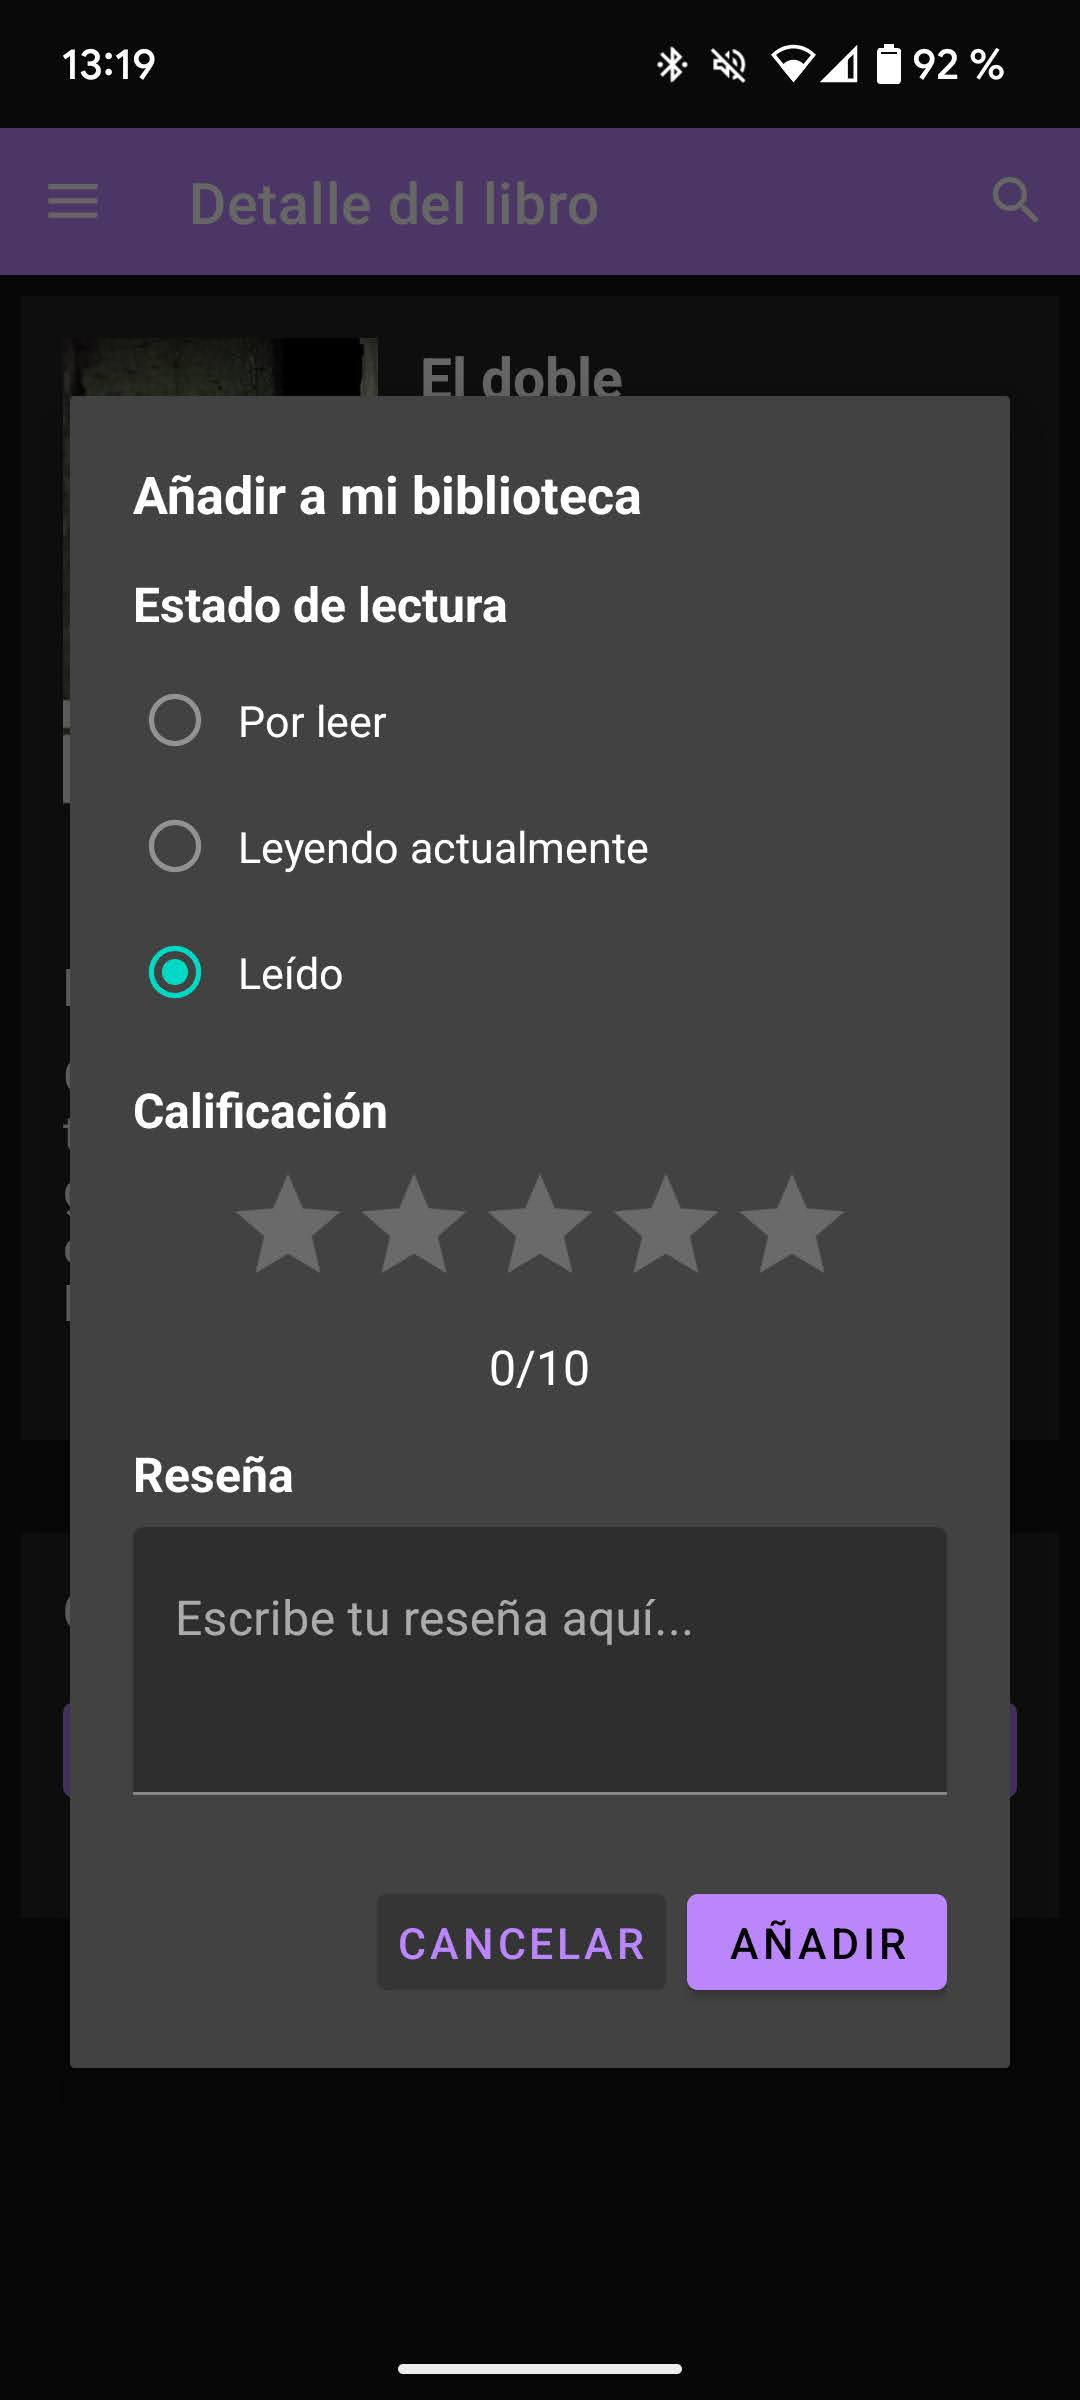
\includegraphics[width=0.47\linewidth]{.img/libro-leido.png}\hfill
          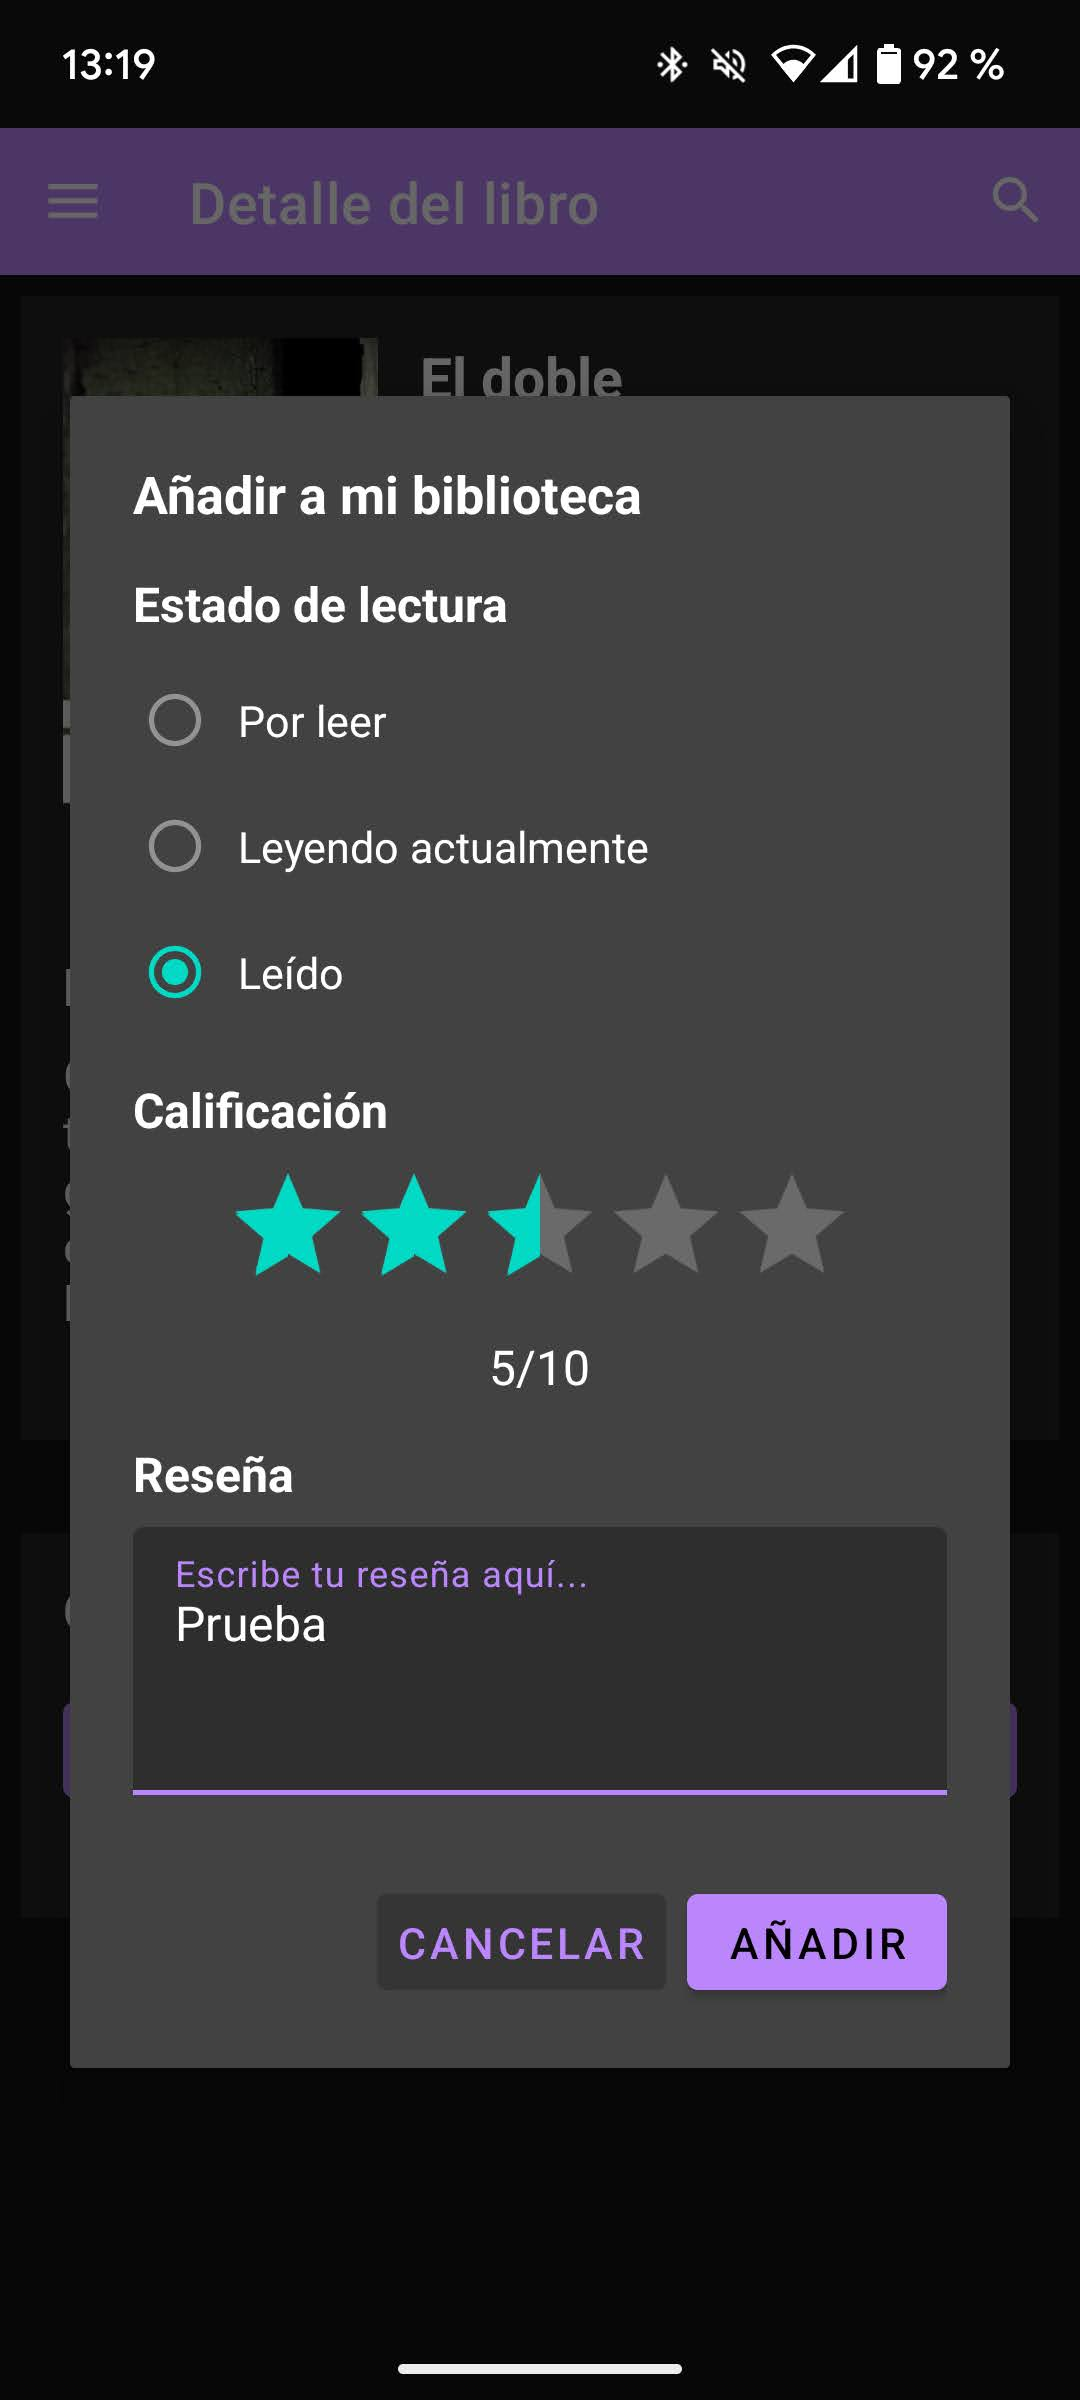
\includegraphics[width=0.47\linewidth]{.img/libro-leido-datos.png}
          \caption{Añadir libro como "Leído" (izq.) y su visualización (der.)}
        \end{figure}
        \vspace{-0.8em}  % Reduce espacio después de la figura
        
        En pantallas grandes o en orientación horizontal, la interfaz se adapta para mostrar más información.
        
        \begin{figure}[H]
          \centering
          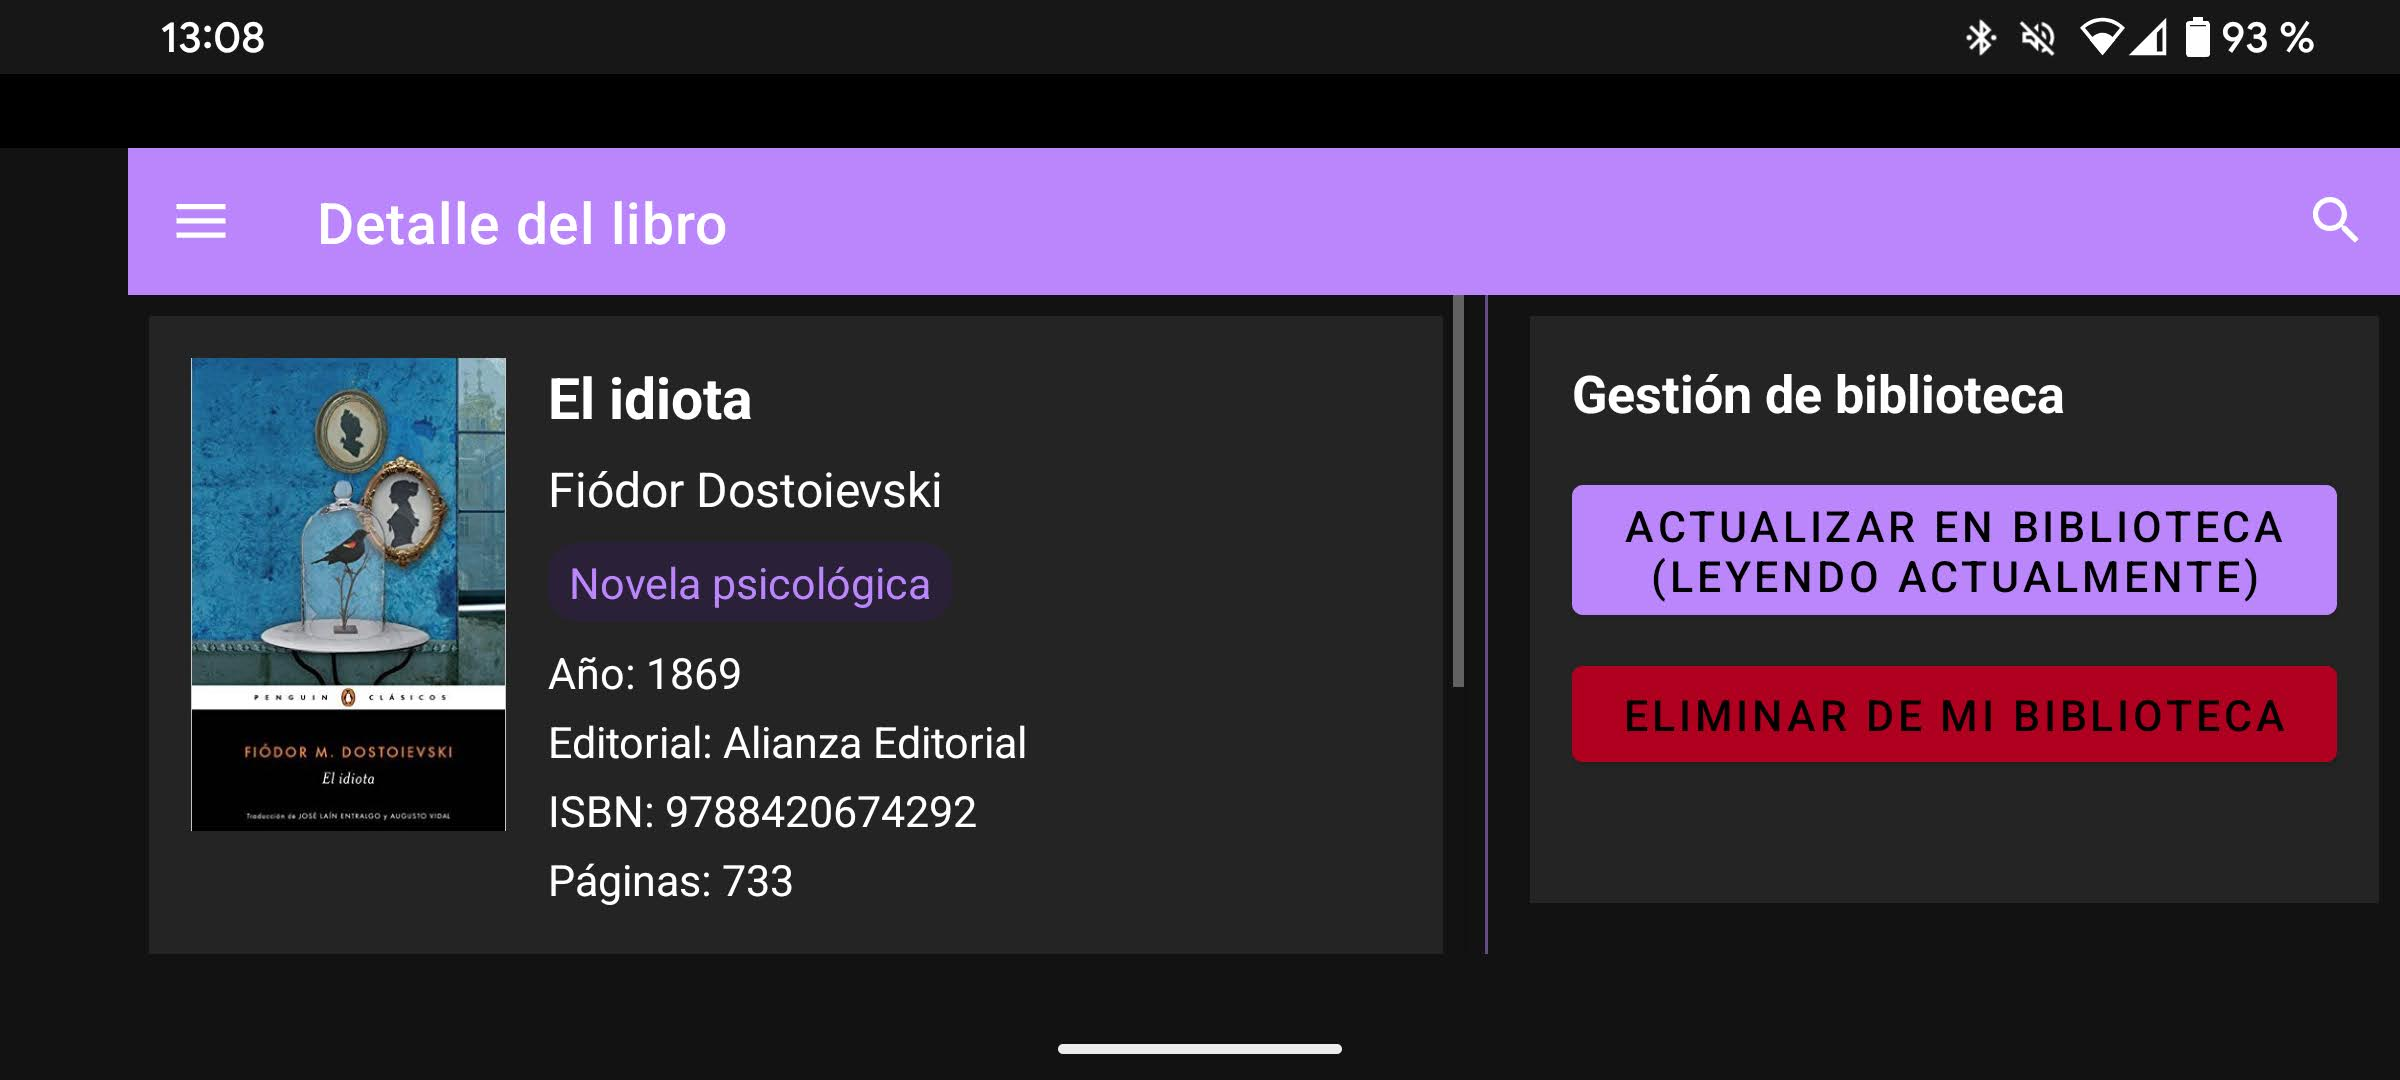
\includegraphics[width=0.95\linewidth]{.img/libro-land.png}
          \caption{Vista de detalles en horizontal}
        \end{figure}
        \vspace{-0.8em}  % Reduce espacio después de la figura
        
        \section{Ajustes y cierre de sesión}
        \vspace{-0.8em}  % Reduce espacio después del título
        Puedes configurar el idioma (inglés, español o euskera) y el tema de la aplicación (claro, oscuro o sistema).
        
        \begin{figure}[H]
          \centering
          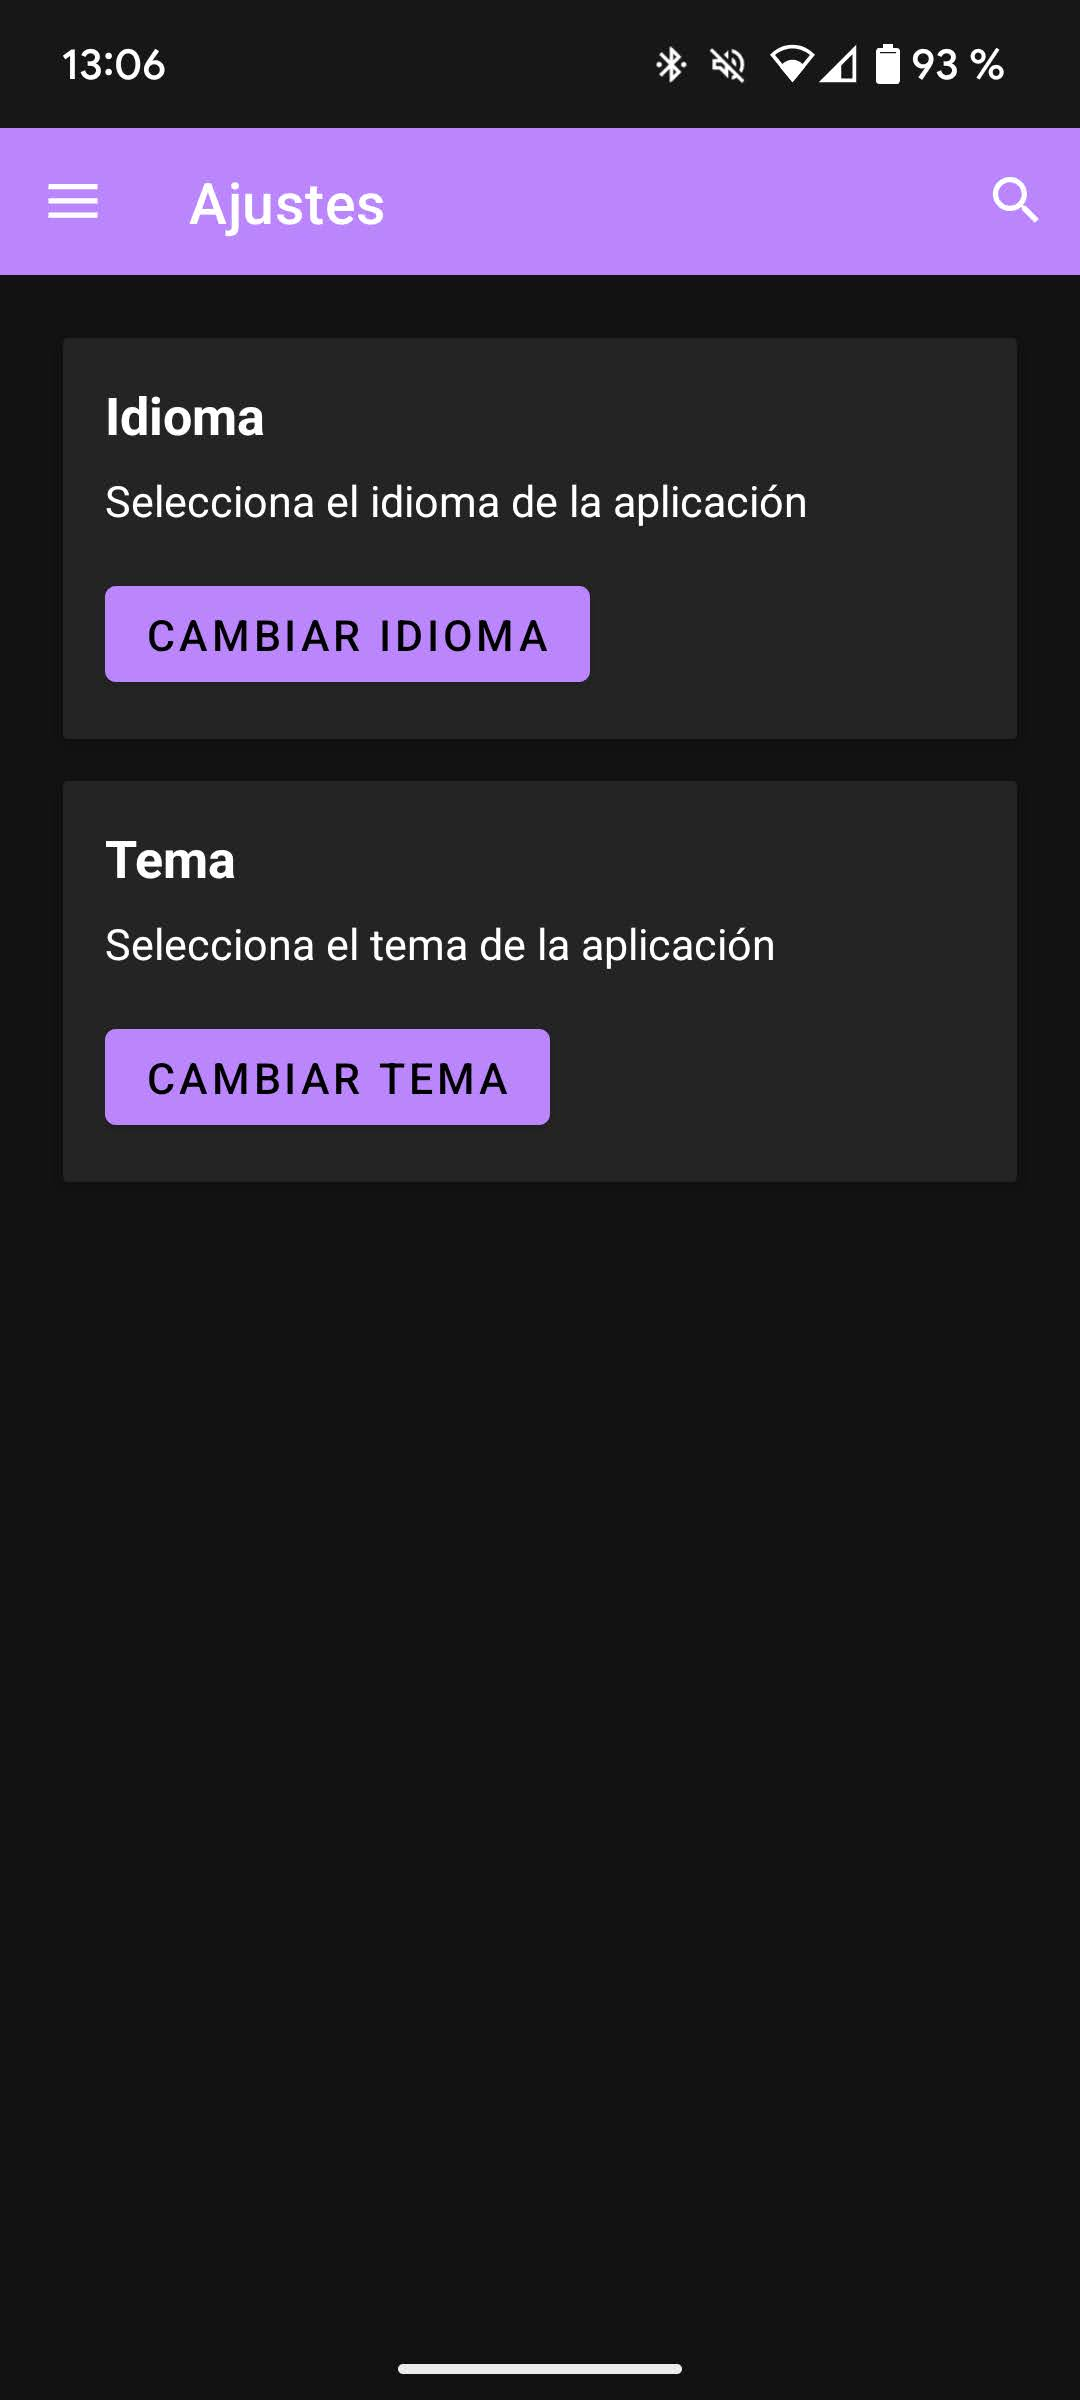
\includegraphics[width=0.47\linewidth]{.img/ajustes.png}\hfill
          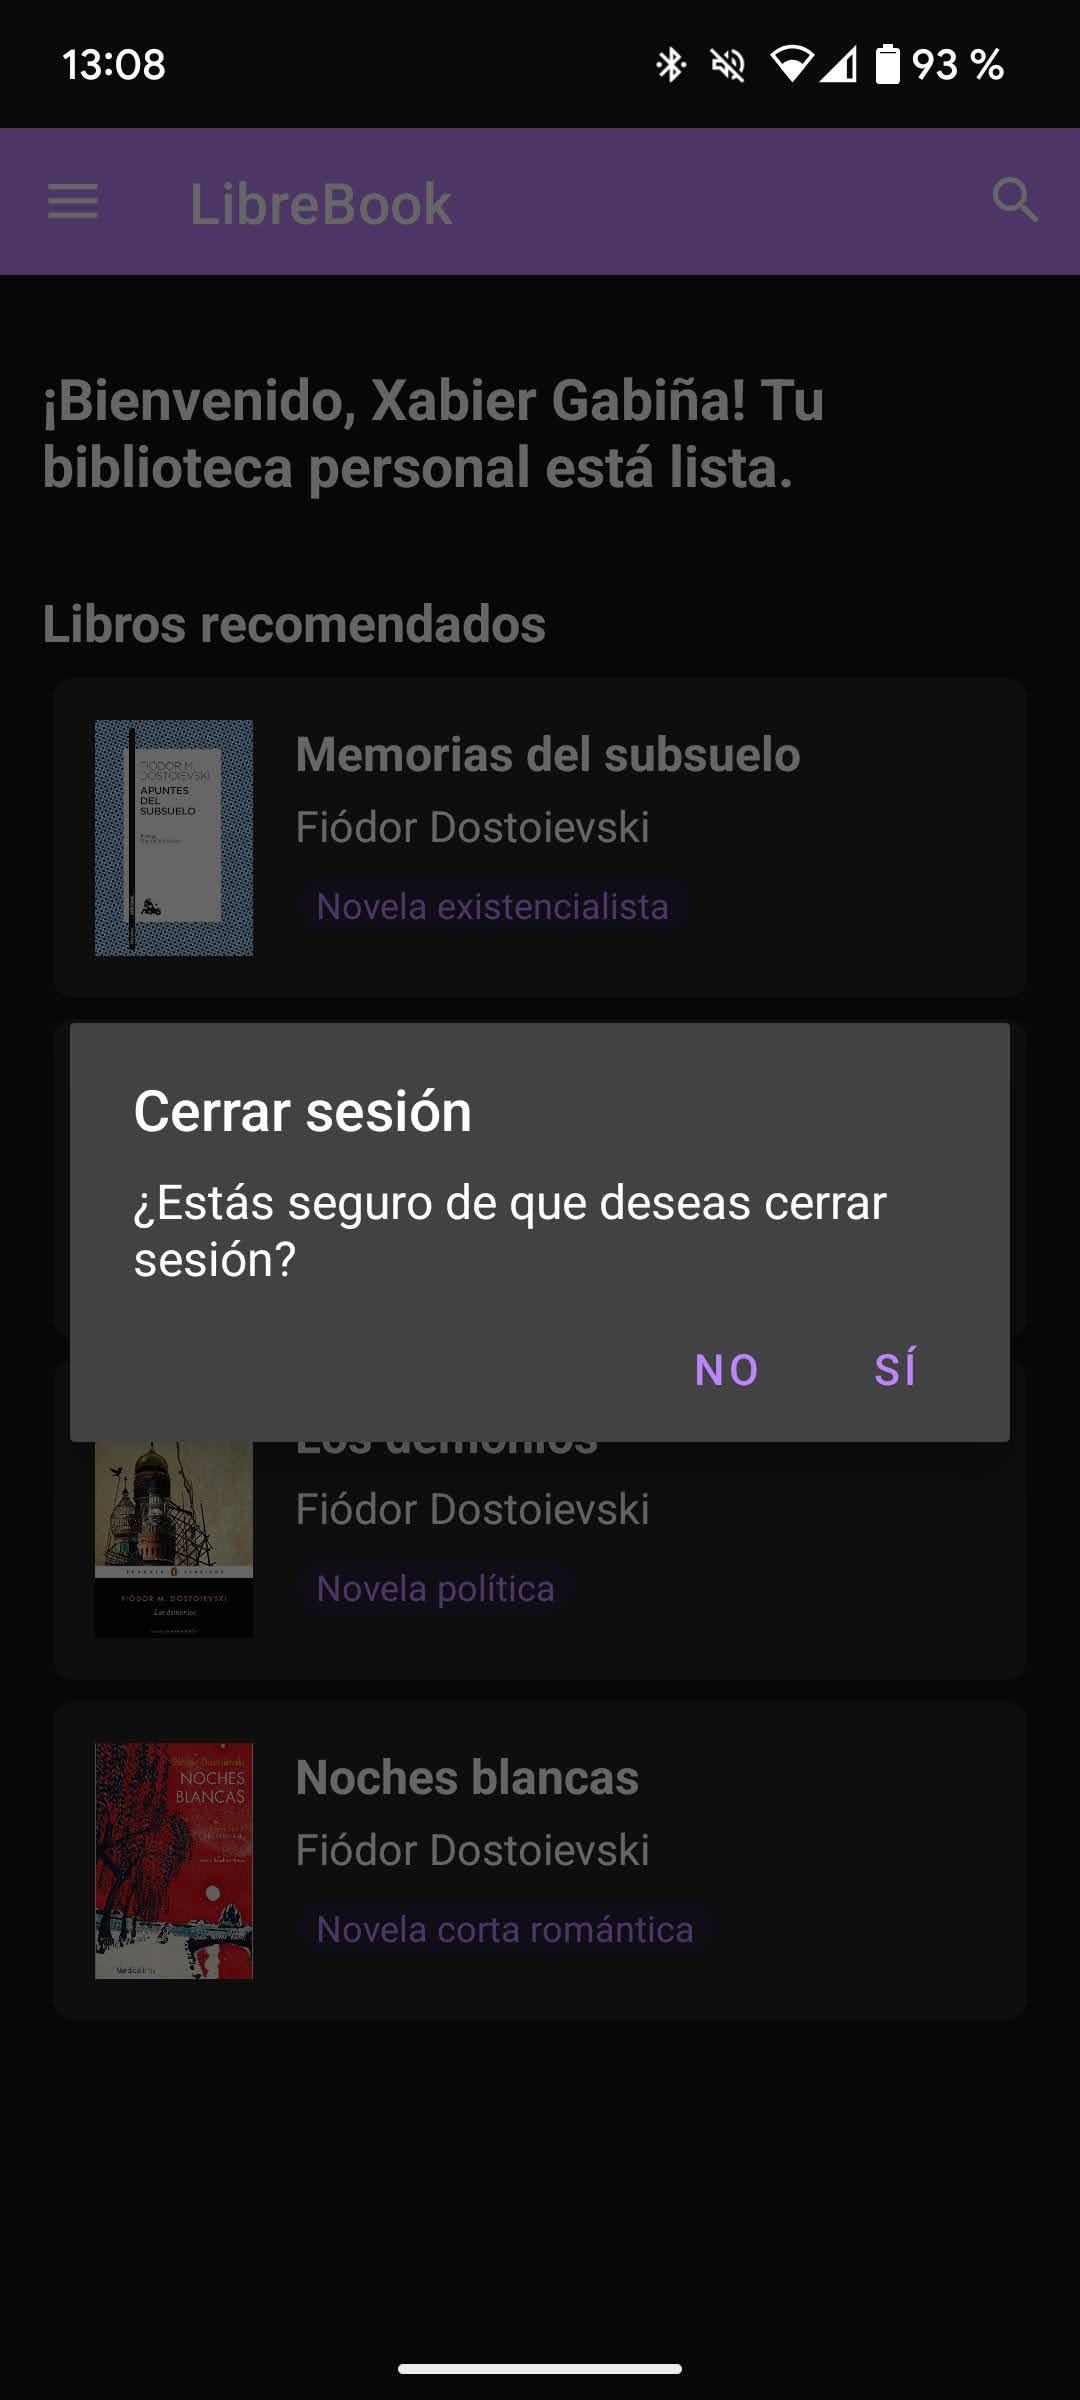
\includegraphics[width=0.47\linewidth]{.img/logout.png}
          \caption{Ajustes (izq.) y diálogo de cierre de sesión (der.)}
        \end{figure}
        \end{multicols}   
  \chapter{Dificultades}
  \chapter{Conclusiones}
\end{document}